 \documentclass[12pt]{book}
%https://www.overleaf.com/project/629e18789b6baeb860fd2545
%\usepackage[numbers]{natbib} % Tidies up citation numbers.

\usepackage[utf8]{inputenc}
\usepackage[backend=biber,backref=true,style=abnt,natbib=true,repeatfields=true,pretty=true,noslsn=true]{biblatex}
%\usepackage[backend=biber,style=abnt,natbib=true,refsegment=chapter,backref=true,backrefstyle=three,repeatfields=true,pretty=true,noslsn=true]{biblatex}
\usepackage{csquotes}

\usepackage{graphicx}
\usepackage{pythonhighlight}
\usepackage{listingsutf8}
\usepackage{float}

%\def\UrlBreaks{\do\/\do-}
\usepackage[T1]{fontenc}
\usepackage{url}[hyphens]
%\usepackage[anythingbreaks]{breakurl}

\usepackage{pdfpages}

\lstset{
  extendedchars=true,
  language=java,
  basicstyle=\tiny\ttfamily,
  showspaces=false,
  showstringspaces=false,
    literate=
     {É}{{\'E}}{1}%
      {Á}{{\'A}}{1}%
      {Ã}{{\~A}}{1}%
      {Â}{{\^A}}{1}%
      {À}{{\`A}}{1}%
      {Ç}{{\,C}}{1}%
      {Ó}{{\'O}}{1}%
      {Í}{{\'I}}{1}%
      {Õ}{{\~O}}{1}%
      {Ú}{{\'U}}{1}%
      {ú}{{\'u}}{1}%
      {é}{{\'e}}{1}%
      {á}{{\'a}}{1}%
      {ã}{{\~a}}{1}%
      {à}{{\`a}}{1}%
      {â}{{\^a}}{1}%
      {ç}{{\,c}}{1}%
      {ó}{{\'o}}{1}%
      {í}{{\'i}}{1}%
      {õ}{{\~o}}{1}%
}

\lstset{
  extendedchars=true,
  language=python,
  basicstyle=\tiny\ttfamily,
  showspaces=false,
  showstringspaces=false,
    literate=
     {É}{{\'E}}{1}%
      {Á}{{\'A}}{1}%
      {Ã}{{\~A}}{1}%
      {Â}{{\^A}}{1}%
      {À}{{\`A}}{1}%
      {Ç}{{\,C}}{1}%
      {Ó}{{\'O}}{1}%
      {Í}{{\'I}}{1}%
      {Õ}{{\~O}}{1}%
      {Ú}{{\'U}}{1}%
      {ú}{{\'u}}{1}%
      {é}{{\'e}}{1}%
      {á}{{\'a}}{1}%
      {ã}{{\~a}}{1}%
      {à}{{\`a}}{1}%
      {â}{{\^a}}{1}%
      {ç}{{\,c}}{1}%
      {ó}{{\'o}}{1}%
      {í}{{\'i}}{1}%
      {õ}{{\~o}}{1}%
}

\definecolor{gray}{rgb}{0.4,0.4,0.4}
\definecolor{darkblue}{rgb}{0.0,0.0,0.6}
\definecolor{cyan}{rgb}{0.0,0.6,0.6}

\lstdefinelanguage{XML}
{
 numbers=left,
 numberstyle=\tiny,
 stepnumber=1,
 numbersep=8pt,
 morestring=[b]",
 morestring=[s]{>}{<},
 morecomment=[s]{<?}{?>},
 stringstyle=\color{black},
 identifierstyle=\color{darkblue},
 keywordstyle=\color{cyan},
 morekeywords={xmlns,version,type}% list your attributes here
}

\colorlet{punct}{red!60!black}
\definecolor{background}{HTML}{EEEEEE}
\definecolor{delim}{RGB}{20,105,176}
\colorlet{numb}{magenta!60!black}

\lstdefinelanguage{json}{
    basicstyle=\tiny\ttfamily,
    numbers=left,
    numberstyle=\tiny,
    stepnumber=1,
    numbersep=8pt,
    showstringspaces=false,
    breaklines=true,
    frame=lines,
    backgroundcolor=\color{background},
    literate=
     *{É}{{\'E}}{1}%
      {Á}{{\'A}}{1}%
      {Ã}{{\~A}}{1}%
      {Â}{{\^A}}{1}%
      {À}{{\`A}}{1}%
      {Ç}{{\,C}}{1}%
      {Ó}{{\'O}}{1}%
      {Í}{{\'I}}{1}%
      {Õ}{{\~O}}{1}%
      {Ú}{{\'U}}{1}%
      {ú}{{\'u}}{1}%
      {é}{{\'e}}{1}%
      {á}{{\'a}}{1}%
      {ã}{{\~a}}{1}%
      {à}{{\`a}}{1}%
      {â}{{\^a}}{1}%
      {ç}{{\,c}}{1}%
      {ó}{{\'o}}{1}%
      {í}{{\'i}}{1}%
      {õ}{{\~o}}{1}%
     {0}{{{\color{numb}0}}}{1}
      {1}{{{\color{numb}1}}}{1}
      {2}{{{\color{numb}2}}}{1}
      {3}{{{\color{numb}3}}}{1}
      {4}{{{\color{numb}4}}}{1}
      {5}{{{\color{numb}5}}}{1}
      {6}{{{\color{numb}6}}}{1}
      {7}{{{\color{numb}7}}}{1}
      {8}{{{\color{numb}8}}}{1}
      {9}{{{\color{numb}9}}}{1}
      {:}{{{\color{punct}{:}}}}{1}
      {,}{{{\color{punct}{,}}}}{1}
      {\{}{{{\color{delim}{\{}}}}{1}
      {\}}{{{\color{delim}{\}}}}}{1}
      {[}{{{\color{delim}{[}}}}{1}
      {]}{{{\color{delim}{]}}}}{1},
}

\lstdefinelanguage{SPARQL}{
    basicstyle=\tiny\ttfamily,
    numbers=left,
    numberstyle=\tiny,
    stepnumber=1,
    numbersep=8pt,
    showstringspaces=false,
    breaklines=true,
    frame=lines,
    backgroundcolor=\color{background},
    literate=
     {É}{{\'E}}{1}%
      {Á}{{\'A}}{1}%
      {Ã}{{\~A}}{1}%
      {Â}{{\^A}}{1}%
      {À}{{\`A}}{1}%
      {Ç}{{\,C}}{1}%
      {Ó}{{\'O}}{1}%
      {Í}{{\'I}}{1}%
      {Õ}{{\~O}}{1}%
      {Ú}{{\'U}}{1}%
      {ú}{{\'u}}{1}%
      {é}{{\'e}}{1}%
      {á}{{\'a}}{1}%
      {ã}{{\~a}}{1}%
      {à}{{\`a}}{1}%
      {â}{{\^a}}{1}%
      {ç}{{\,c}}{1}%
      {ó}{{\'o}}{1}%
      {í}{{\'i}}{1}%
      {õ}{{\~o}}{1},%
  morekeywords={
    SELECT,CONSTRUCT,DESCRIBE,ASK,WHERE,FROM,NAMED,PREFIX,BASE,OPTIONAL,
    FILTER,GRAPH,LIMIT,OFFSET,SERVICE,UNION,EXISTS,NOT,BINDINGS,MINUS,a
  }
}

\lstdefinelanguage{overpassQL}{
    basicstyle=\tiny\ttfamily,
    numbers=left,
    numberstyle=\tiny,
    stepnumber=1,
    numbersep=8pt,
    showstringspaces=false,
    breaklines=true,
    frame=lines,
    backgroundcolor=\color{background}
}

\lstset{language=R,
    literate=
    {<-}{{$\gets$}}1%
     {É}{{\'E}}{1}%
     {Ê}{{\^E}}{1}%
      {Á}{{\'A}}{1}%
      {Ã}{{\~A}}{1}%
      {Â}{{\^A}}{1}%
      {À}{{\`A}}{1}%
      {Ç}{{\,C}}{1}%
      {Ó}{{\'O}}{1}%
      {Í}{{\'I}}{1}%
      {Õ}{{\~O}}{1}%
      {Ú}{{\'U}}{1}%
      {ú}{{\'u}}{1}%
      {ê}{{\^e}}{1}%
      {é}{{\'e}}{1}%
      {á}{{\'a}}{1}%
      {ã}{{\~a}}{1}%
      {à}{{\`a}}{1}%
      {â}{{\^a}}{1}%
      {ç}{{\,c}}{1}%
      {ó}{{\'o}}{1}%
      {í}{{\'i}}{1}%
      {õ}{{\~o}}{1},%
    basicstyle=\tiny\ttfamily,
    stringstyle=\color{red},
    otherkeywords={0,1,2,3,4,5,6,7,8,9},
    morekeywords={TRUE,FALSE},
    deletekeywords={data,frame,length,as,character},
    keywordstyle=\color{blue},
    commentstyle=\color{red},
}

\usepackage[brazil]{babel}  
\usepackage{xcolor}
%xcolor v2.12 (2016/05/11)384  Colors by Name4.1  Base colors (always available)black blue brown cyan darkgray gray green lightgray lime magenta olive orange pink purple red teal violet white yellow

\PassOptionsToPackage{hyphens}{url}
\usepackage [colorlinks = true,
            linkcolor = blue,
            urlcolor  = blue,
            citecolor = blue,
            anchorcolor = blue]{hyperref} 

\usepackage[nopostdot]{glossaries}
\setglossarystyle{altlist}

% gerador de lero-lero
\usepackage{lipsum}

\newenvironment{itquote}
{\begin{quote}\itshape}
{\end{quote}}

\usepackage[todonotes={textsize=footnotesize,portuguese}]{changes}

\presetkeys%
    {todonotes}%
    {inline,backgroundcolor=yellow}{}
\usepackage{datetime2}

\usepackage{booktabs}

\usepackage{siunitx,array}

\usepackage{caption}

\usepackage{csvsimple} % para leitura de arquivos csv

\usepackage{fancyhdr,ragged2e}
\fancyhead{}
\lhead{\parbox[t]{0.35\textwidth}{\RaggedRight\rightmark\strut}}
\rhead{\parbox[t]{0.63\textwidth}{\RaggedLeft\leftmark\strut}}
\setlength{\headheight}{5\baselineskip}

\usepackage
%[final]
{changes}
%\usepackage{changes}
%\url{https://ctan.org/pkg/changes}


\usepackage{wrapfig}
\usepackage{longtable}
\usepackage{booktabs}


% define cores personalizadas para o texto de cada autor
\definechangesauthor[name={Jorge Henrique Cabral Fernandes}, color=orange]{jhcf} % git-user: jhcf
\definechangesauthor[name={Gabriel da Silva Corvino Nogueira}, color=orange]{nosgueira} % git-user: nosgueira
\definechangesauthor[name={Gabriel Ligoski}, color=blue]{gabrielligoski} % git-user: gabrielligoski
\definechangesauthor[name={Gustavo Rodrigues Gualberto}, color=green]{GustavoRGYGO} % git-user: GustavoRGYGO
\definechangesauthor[name={Edgar Sampaio de Barros}, color=green]{edgarsamp} % git-user: edgarsamp
\definechangesauthor[name={Erick Rodrigues Fraga}, color=green]{mutenesss} % git-user: mutenesss
\definechangesauthor[name={João Pedro de Sousa Soares Martins}, color=green]{jpssm} % git-user: jpssm
\definechangesauthor[name={Thiago Masera Tokarski}, color=green]{Toskosz} % git-user: Toskosz
\definechangesauthor[name={Marcelo Aiache Postiglione}, color=green]{marcelo3101} % git-user: marcelo3101
\definechangesauthor[name={Arthur Barreiros de Oliveira Mota}, color=purple]{BarreirosM} % git-user: BarreirosM
\definechangesauthor[name={Weliton César Pereira Barreto}, color=red]{welitonbarreto} % git-user: welitonbarreto
\definechangesauthor[name={Gabriel Pinheiro da Conceicao}, color=blue]{pinheirogh} % git-user: pinheirogh
\definechangesauthor[name={Breno Ribeiro Corrêa}, color=red]{brenoZ} % git-user: brenoZ
\definechangesauthor[name={João Victor de Souza Calassio}, color=blue]{jvcalassio} % git-user: jvcalassio
\definechangesauthor[name={Matheus Barbosa Santos}, color=cyan]{MatBSa} % git-user: MatBSa
\definechangesauthor[name={Plínio Candide Rios Mayer}, color=green]{PlinioMayer} % git-user: PlinioMayer
\definechangesauthor[name={Marco Antonio Nemetala Garcia}, color=green]{Hadeshade} % git-user: Hadeshade
\definechangesauthor[name={Regina Emy Da Nobrega Kamada}, color=orange]{bananaMoshpit} % git-user: bananaMoshpit
\definechangesauthor[name={Felipe Gomes Paradas}, color=purple]{fparadas} % git-user: fparadas
\definechangesauthor[name={Paulo Alvim Alvarenga}, color=yellow]{alvimpaulo} % git-user: alvimpaulo
\definechangesauthor[name={Marco Antônio Souza de Athayde}, color=pink]{masathayde} % git-user: masathayde
\definechangesauthor[name={João Antônio Desiderio de Moraes}, color=green]{joaoadm94} % git-user: joaoadm94
\definechangesauthor[name={Lucas de Oliveira Silva}, color=pink]{LuscasOSilva} % git-user: LuscasOSilva
\definechangesauthor[name={Isaque Augusto da Silva Santos}, color=pink]{seraphritt} % git-user: seraphritt
\definechangesauthor[name={Claudio Roberto Oliveira Peres de Barros}, color=pink]{ClaudioBarros} % git-user: ClaudioBarros
\definechangesauthor[name={André Cássio Barros de Souza}, color=pink]{andreloff} % git-user: andreloff
\definechangesauthor[name={Fernando Ferreira Cordeiro}, color=green]{FernandoCordeiro} % git-user: FernandoCordeiro
\definechangesauthor[name={Paulo Mauricio Costa Lopes}, color=orange]{RequiemDosVivos} % git-user: RequiemDosVivos
\definechangesauthor[name={Bruno Abreu Kamienski}, color=magenta]{brunosabreu} % git-user: brunosabreu
\definechangesauthor[name={André Fioravante Nicolodi Durante Júnior}, color=green]{AndreDuranteJr} % git-user: Andredurantejr

\definechangesauthor[name={Gabriel Teixeira Ribeiro}, color=blue]{moltentheory} % git-user: moltentheory

%MILLER, John H.; PAGE, Scott E. Complex Adaptive Systems: An introduction to computational models of social life. USA: Princeton University Press, 2007.


 

\makenoidxglossaries
\loadglsentries{1-Introducao/tarefas/T2-Glossario/estudantes/main}

\setcounter{tocdepth}{5}
\setcounter{secnumdepth}{5}
%\captionsetup[table]{name=Quadro}
\renewcommand{\lstlistingname}{Listagem de Código}

\newcommand{\dataset}{\textit{dataset}}
\newcommand{\query}{\textit{query}}
\newcommand{\githubusername}{\textless githubusername\textgreater}

\def\printpart{1} % Orientações Gerais, Introdução e Fundamentos de Pesquisa Bibliográfica

% Substitua o valor de printpart por 1, 2, 3, 4 ou 5, conforme a parte do documento que você quer gerar 
\def\printpart{1}

\setlength{\headheight}{73.04742pt}
\addtolength{\oddsidemargin}{-1.5cm}
\addtolength{\evensidemargin}{-1.5cm}
\addtolength{\textwidth}{3cm}
\addtolength{\topmargin}{-3cm}
\addtolength{\textheight}{2cm}

\addbibresource{RESIC.bib}
	
\begin{document}
\pagenumbering{gobble}% Remove page numbers (and reset to 1)
\clearpage
\thispagestyle{empty}

\begin{titlepage}
\begin{center}
 {\huge\bfseries 
\includegraphics[width=4cm]{unb-logo.jpg}\\
	CIC0203 - Computação Experimental - TA - 2022.2 - Notas e Registros
	\\Overleaf read only: \url{https://www.overleaf.com/read/rytgshjfsgpv}\\ 
	Github Repositório Origin (enviar tarefas aqui): \url{https://github.com/jhcf/Comput-Experim-20222}\\
	}

 % ----------------------------------------------------------------
 \vspace{1.5cm}
{\large	% author names and affiliations
	Jorge Henrique Cabral Fernandes (jhcf)\\
	Arthur Barreiros de Oliveira Mota (BarreirosM)\\
    Gabriel Pinheiro da Conceição (pinheirogh)\\
    Breno Ribeiro Corrêa (brenoZ)\\
    João Victor de Souza Calassio (jvcalassio)\\
    Matheus Barbosa Santos (MatBSa)\\
    Edgar Sampaio de Barros (edgarsamp) \\
    Felipe Gomes Paradas (fparadas) \\
    Marcelo Aiache Postiglione (marcelo3101) \\
    Paulo Alvim Alvarenga (alvimpaulo)\\
    Marco Antônio Souza de Athayde (masathayde)\\
    João Antonio Desidério de Moraes (joaoadm94)\\
    Gabriel da Silva Corvino Nogueira (nosgueira)\\
    Thiago Masera Tokarski (Toskosz)\\
    Erick Rodrigues Fraga (mutenesss)\\
    André Cássio Barros de Souza (andreloff)\\
    Lucas de Oliveira Silva (LuscasOSilva)\\
    João Pedro de Sousa Soares Martins (jpssm)\\
	Isaque Augusto da Silva Santos (seraphritt)\\
	Gustavo Rodrigues Gualberto (GustavoRGYGO)\\
    André Fioravante Nicolodi Durante Júnior (AndreDuranteJr)\\
	Cláudio Roberto Oliveira Peres de Barros (ClaudioBarros)\\ 
        Fernando Ferreira Cordeiro (FernandoCordeiro)\\
        Paulo Mauricio Costa Lopes (RequiemDosVivos)\\
	Bruno Abreu Kamienski (brunosabreu)\\
	Gabriel Teixeira Ribeiro\\
 }
	\vspace{1.5cm}
	{\large Brasília, \DTMnow}
\end{center}
\end{titlepage}
	%\date{10 de março de 2021}
	% make the title area
    %\maketitle
    \listoftodos
	\printnoidxglossary
	\tableofcontents
	\listoffigures
	\listoftables
	\clearpage
\pagenumbering{arabic}

\pagestyle{fancy}

	\chapter*{Resumo}

	Este documento contém notas de aula e registros em geral, produzidos de forma textual, pelo professor e turma da disciplina CIC0203 - Computação Experimental - TA - 2022.2.
	
	A disciplina adotará a abordagem de estudos estatísticos de simulações computacionais, como base para a construção de experimentos.

\part{Preparação\label{part:intro}}

    \chapter{Manipulação de Variáveis em Simulações}

Neste capítulo você aprenderá a projetar e codificar a manipulação de variáveis no seu modelo de simulação, que posteriormente serão consideradas variáveis independentes ou de controle de um experimento.



    \chapter{Tarefa 9 - Teste Estatístico de Hipóteses e Estudos de Caso - Parte 2. 30 pontos\label{tarefa:teste:hipotese2:R}}

Antes de realizar essa tarefa, veja atentamente as instruções do capítulo anterior: "Conceitos Centrais em Estatística Inferencial".

Nessa tarefa você vai criar um novo capítulo, a partir do refinamento do capítulo anterior onde descreveu o seu laboratório com o teste para variáveis categóricas. Depois, vai fazer uma apresentação oral do seu capítulo em vídeo, conforme as orientações a seguir.
%como no modelo da seção \ref{tarefa:teste:hipotese:R:jhcf}, contendo um %texto com as seguintes características:

\section{Revise o texto da tarefa anterior}

Revise cuidadosamente todo o texto da tarefa anteriormente realizada, para que nada do que foi solicitado fique ausente.

\section{Teste do Chi-Quadrado} 

O teste do Chi-Quadrado permite explorar a chance de associação não aleatória entre dados categóricos, na forma de uma tabela crosstable. Crie uma seção que explora, declara e verifica hipóteses usando esse tipo de teste, com os dados de seu experimento. Adote como exemplo o código da listagem a seguir.

 \lstinputlisting[numbers=left,language={R},basicstyle=\tiny\ttfamily,caption={Realizando um teste de chi quadrado com amostras de um experimento},label={code:jhf:X2testCode}]{4-Computacao-Experimental/tarefas/T9-Teste-Hipoteses2/chi-square.R}
 
\section{Estudo de Caso}

Adote a abordagem de estudo de caso, para analise e descrição da evolução de um único experimento executado no seu simulador, desde o início até o alcance de estabilidade do fenômeno. Ao final, caracterize o experimento como sendo um caso típico ou de situação extrema, conforme as análises anteriores.

Crie uma seção chamada Estudo de Caso, para conter sua descrição.
Use pelo menos 250 palavras para essa seção.  

\section{Ética}

Vídeos e site:
\begin{description}
    \item [\url{https://www.youtube.com/watch?v=thbKYoLN1Ek}]
    \item [\url{https://www.youtube.com/watch?v=p6Ls45MVETk}]
    \item [Plataforma Brasil] \url{https://plataformabrasil.saude.gov.br/login.jsf}
\end{description}

Conforme os seus conhecimento de ética na realização de experimentos, discorra sobre as implicações éticas da realização de experimentos no mundo real, relativos ao fenômeno investigado.
Use pelo menos 250 palavras para essa seção.  

\section{Apresentação em Vídeo}
 
 Faça uma gravação da apresentação em vídeo do seu capítulo, nas reuniões de nomes "Apresentações em Vídeo A", "Apresentações em Vídeo B" ou "Apresentações em Vídeo C", disponíveis no ambiente Teams da disciplina, contendo os seguintes aspectos:
 \begin{description}
     \item [Seu rosto] Inicie apresentando o seu rosto, seu nome e dizendo o que contém o vídeo: "Uma apresentação do seu laboratório";
     \item [Texto] Compartilhe o texto do seu capítulo, para conduzir o restante da apresentação;
     \item [Execução do simulador] Apresente o seu simulador em execução interativa, mostrando como ele pode ser usado de forma prática; e
     \item [Hipóteses e resultados dos testes] Apresente os testes de hipóteses significativamente estatísticas que você fez, e interprete os resultados. 
 \end{description}
Não esqueça de gravar seu vídeo.

O seu vídeo deverá ter entre 5 e 15 minutos de duração.


% \begin{enumerate}
%     \item [Seção Introdução] Revise a apresentação das seções, já que o seu capítulo agora ficou mais extenso; 
%     \item [Seção o ``O Laboratório'']
%     \begin{description}
%     \item [Variáveis independentes ou de controle]
%     Registre e apresente, necessariamente, uma ou mais figuras com a interface  simulador, onde estão presentes as variáveis que podem ser independentes ajustadas, bem como as variáveis dependentes. Para cada variável independente ou de controle, informe se ela é do tipo (\url{https://rcompanion.org/handbook/C_01.html}):
%     \begin{description}
%     \item [nominal] ``Variáveis nominais são aquelas cujos níveis são rótulos ou descrições e que não podem ser ordenados. Exemplos de variáveis nominais são sexo, escola e perguntas sim/não. Eles também são chamados de variáveis “categóricas nominais” ou “qualitativas”, e os níveis de uma variável são às vezes chamados de “classes” ou “grupos”''
%     \item [ordinal] ``As variáveis ordinais são aquelas cujos valores podem ser ordenados ou classificados em ordem lógica, mas o intervalo entre os níveis das variáveis não é necessariamente conhecido. Medidas subjetivas são frequentemente variáveis ordinais. Um exemplo seria fazer com que as pessoas classificassem quatro itens por preferência em ordem de um a quatro. Um exemplo diferente seria fazer com que as pessoas avaliassem vários itens com base em uma escala de classificação Likert: “Em uma escala de um a cinco, você concorda ou discorda dessa afirmação?”. Um terceiro exemplo é o nível de escolaridade para adultos, considerando, por exemplo, “menor que o ensino médio”, “ensino médio”, “superior”, etc.''
%     \item [intervalar] ``As variáveis de intervalo ou razão são aquelas que representam valores medidos ou contados: idade, altura, peso, número de alunos. Sabe-se que o intervalo entre os números é igual: o intervalo entre um quilograma e dois quilogramas é o mesmo que entre três quilogramas e quatro quilogramas.
%  Os dados de intervalo/proporção também são chamados de dados “quantitativos”.

%     \item [intervalar discreta e contínua] 
% "Variáveis intervalares discretas e contínuas, são uma divisão de dados de intervalo ou razão. Nas intervalares discretas, os valores são necessariamente números inteiros ou outros valores discretos, como população ou contagens de itens. As variáveis intervalares contínuas podem assumir qualquer valor dentro de um intervalo e, portanto, podem ser expressas como decimais. Muitas vezes são quantidades medidas. Por exemplo, em teoria, um peso pode ser medido como 1 kg, 1,01 kg ou 1,009 kg e assim por diante. A idade também pode ser considerada uma variável contínua, embora muitas vezes a tratemos como uma variável discreta, arredondando-a para o aniversário mais recente."
%     \end{description}
%     \item [Código do Simulador]
%     Apresente, no código do seu simulador, as partes que introduzem a aleatoriedade dos fenômenos de interação entre os agentes, e argumente de que forma essa aleatoriedade no código contribui para que as amostras do fenômeno simulado também sejam aleatórias. 
%     \end{description}
    
%     \begin{description}
%         \item [Apresentação das Amostras] Nessa seção, refine o que antes era apenas a apresentação das "Variáveis Dependentes e Independentes", nos seguintes termos: 
%         Descreva cada uma das colunas da planilha de amostras de experimentos por você coletadas, informando:
%         \begin{itemize}
%             \item O nome da variável;
%             \item O que significa a variável;
%             \item Se a variável é para uso interno do simulador, variável de controle no experimento, variável independente ou variável dependente;
%             \item As faixas de valores ou categorias dos registros obtidos, para fins de interpretação dos números (ex: Se umidade = 0, o que isso significa? Se umidade = 1, o que significa?;
%         \end{itemize}
        
%         \item [Primeira Declaração Formal de Hipóteses] Revise o texto da sua primeira declaração formal de hipóteses.
        
%         \item [Aplicação do Teste t] 
%         Revise o texto de aplicação do teste t.
        
%         \item [Segunda Declaração Formal de Hipóteses] Revise o texto da sua segunda declaração formal de hipóteses.
    
%         \item [Aplicação do teste de regressão linear] Revise o texto da aplicação do teste de regressão linear.
        
%         \item [Teste do Chi-Quadrado] 
%         Revise o texto da sua primeira declaração formal de hipóteses.
        
%         Supondo que foi feita a escolha inicial do teste t de Student, para comparar médias entre duas amostras (conjunto de registros) de variável dependente, que foram obtidas a partir de estímulos com diferentes valores para pelo menos uma variável independente, faça uma declaração de hipóteses nula e alternativa para o seu teste. Aplique corretamente os conceitos de hipóteses nula e alternativa, conforme o vídeo sobre Inferência Estatística.
%         \item [Aplicação do Teste t] Use as instruções em \url{https://stat.ethz.ch/R-manual/R-devel/library/stats/html/t.test.html}, e com base no vídeo sobre teste t (\url{https://www.youtube.com/watch?v=AgDC9yoopUA}), apresente duas diferentes execuções do teste, comparando diferentes amostras. Apresente, usando lstlistings, todo o código R usado, os resultados apresentados no Console do R, e sua interpretação dos resultados. Informe sobre a comprovação ou rejeição da hipótese nula;
%         \item [Segunda Declaração Formal de Hipóteses] Supondo que agora vais fazer uma análise de regressão linear, com as mesmas amostras, veja o vídeo e o texto sobre regressão linear em R:
%         \begin{itemize}
%             \item \url{https://www.youtube.com/watch?v=u1cc1r_Y7M0}; e
%             \item \url{https://www.r-tutor.com/elementary-statistics/simple-linear-regression/significance-test-linear-regression}.
%         \end{itemize}
%         Com base nos vídeos, faça uma declaração de hipóteses nula e alternativa para o seu teste, que estabeleça possível relação linear entre uma variável independente e uma dependente. Aplique corretamente os conceitos de hipóteses nula e alternativa.
%         \item [Aplicação do teste de regressão linear] Apresente duas diferentes execuções do teste, comparando diferentes amostras por meio de regressão linear. Apresente todo o código R dos comandos e dos resultados apresentados no Console do R, e sua interpretação dos resultados, sobre a comprovação ou não da hipótese nula;
%         \item [Conclusões] Apresente suas conclusões sobre os testes realizados.
%     \end{description}
%  \end{enumerate}
    
%\chapter{Manipulação de Variáveis em Simulações}

Neste capítulo você aprenderá a projetar e codificar a manipulação de variáveis no seu modelo de simulação, que posteriormente serão consideradas variáveis independentes ou de controle de um experimento.




    \chapter{O que é a Ciência?\label{ciência:o:que:eh}}

Existem várias definições sobre o que é a ciência. Algumas questões sobre essa definição são apresentadas por \citep{fernandes_consideracoes_2021}, cujo texto está reproduzido a seguir. 

A figura \ref{fig:ciencia-filosofia}~ apresenta um mapa conceitual que trata da fundamentação do conceito de ciência e sua relação com a filosofia.
Veja o vídeo da aula de 20 de janeiro de 2022, para mais detalhes.

\begin{figure}[ht]
    \centering
    \caption{Conceitos fundamentais de ciência, e sua relação com a filosofia}
    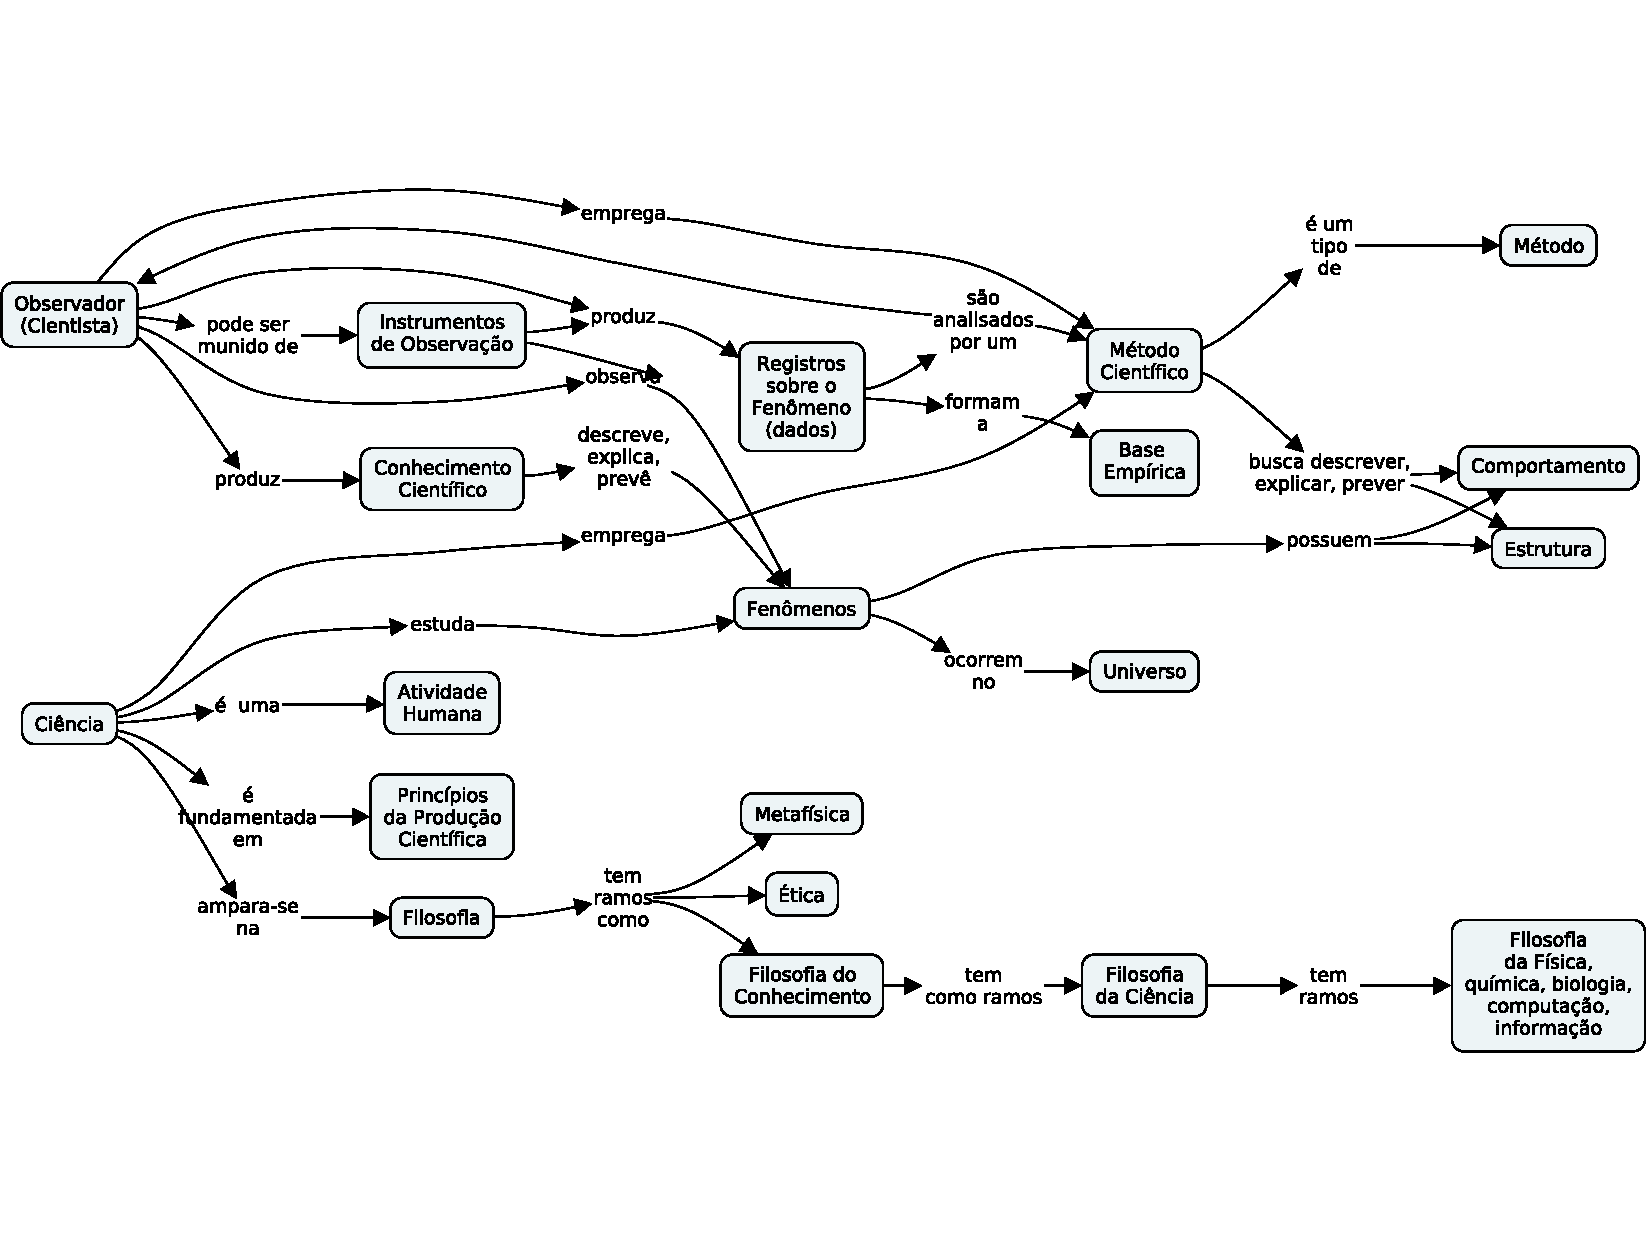
\includegraphics[page=1,angle=90,width=0.9\textwidth,height=0.9\textheight]{1-Introducao/aulas/Ciencia-e-Filosofia.pdf}
    \label{fig:ciencia-filosofia}
\end{figure}

A figura \ref{fig:desenv-sw-ciencia-filosofia} acrescenta à figura  \ref{fig:ciencia-filosofia}~ os conceitos que relacionam a natureza do desenvolvimento de software à  fundamentação do conceito de ciência e sua relação com a filosofia.
Veja o vídeo  da aula de 20 de janeiro de 2022, para mais detalhes.

\begin{figure}[ht]
    \centering
    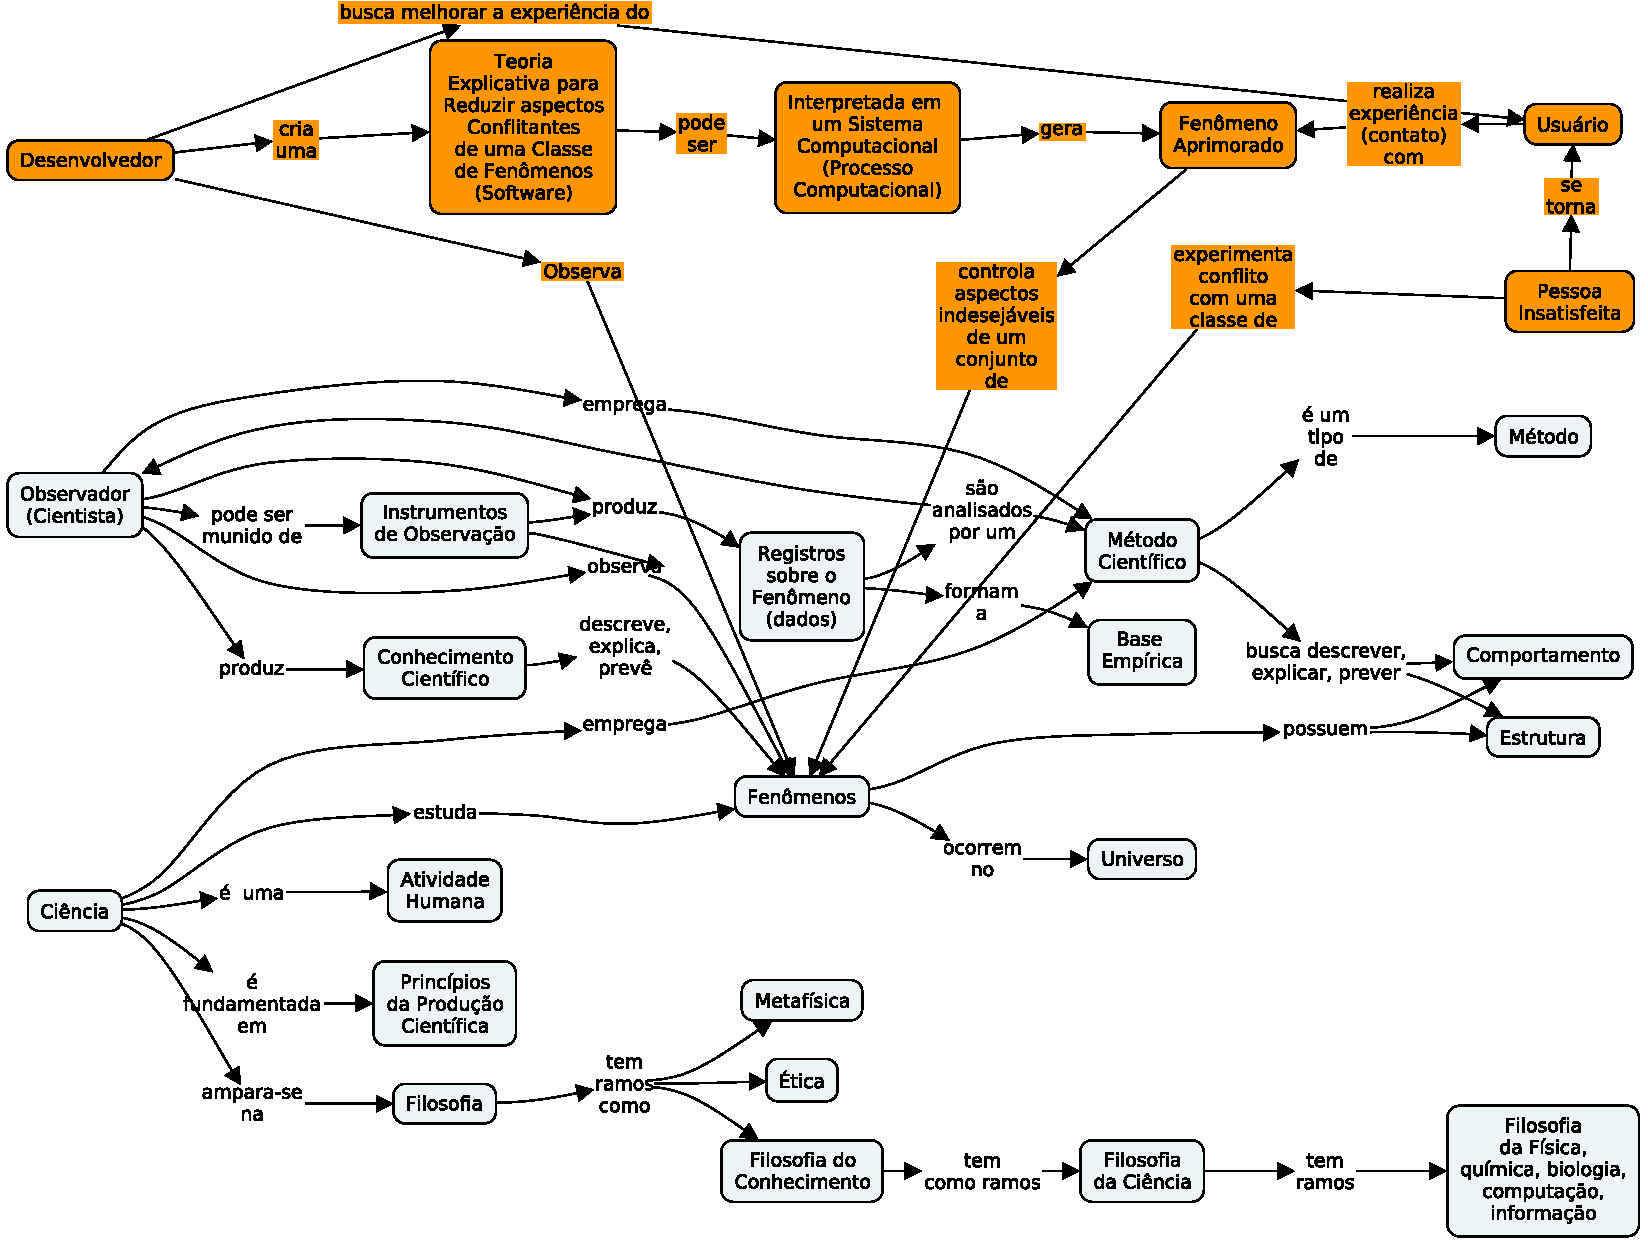
\includegraphics[page=1,angle=90,width=0.8\textwidth,height=0.9\textheight]{1-Introducao/aulas/Desenvolvimento-de-Software-Ciencia-e-Filosofia.pdf}
    \caption{Como a atividade do desenvolvimento de software se compara à atividade cientifica? Fonte: jhcf}
    \label{fig:desenv-sw-ciencia-filosofia}
\end{figure}

A figura \ref{fig:principios:ativ:cientifica}~ sumariza, em um mapa conceitual, os princípios da atividade científica e os relaciona com os princípios do desenvolvimento de software.
Veja o vídeo da aula de 20 de janeiro de 2022, para mais detalhes.

\begin{figure}[ht]
    \centering
    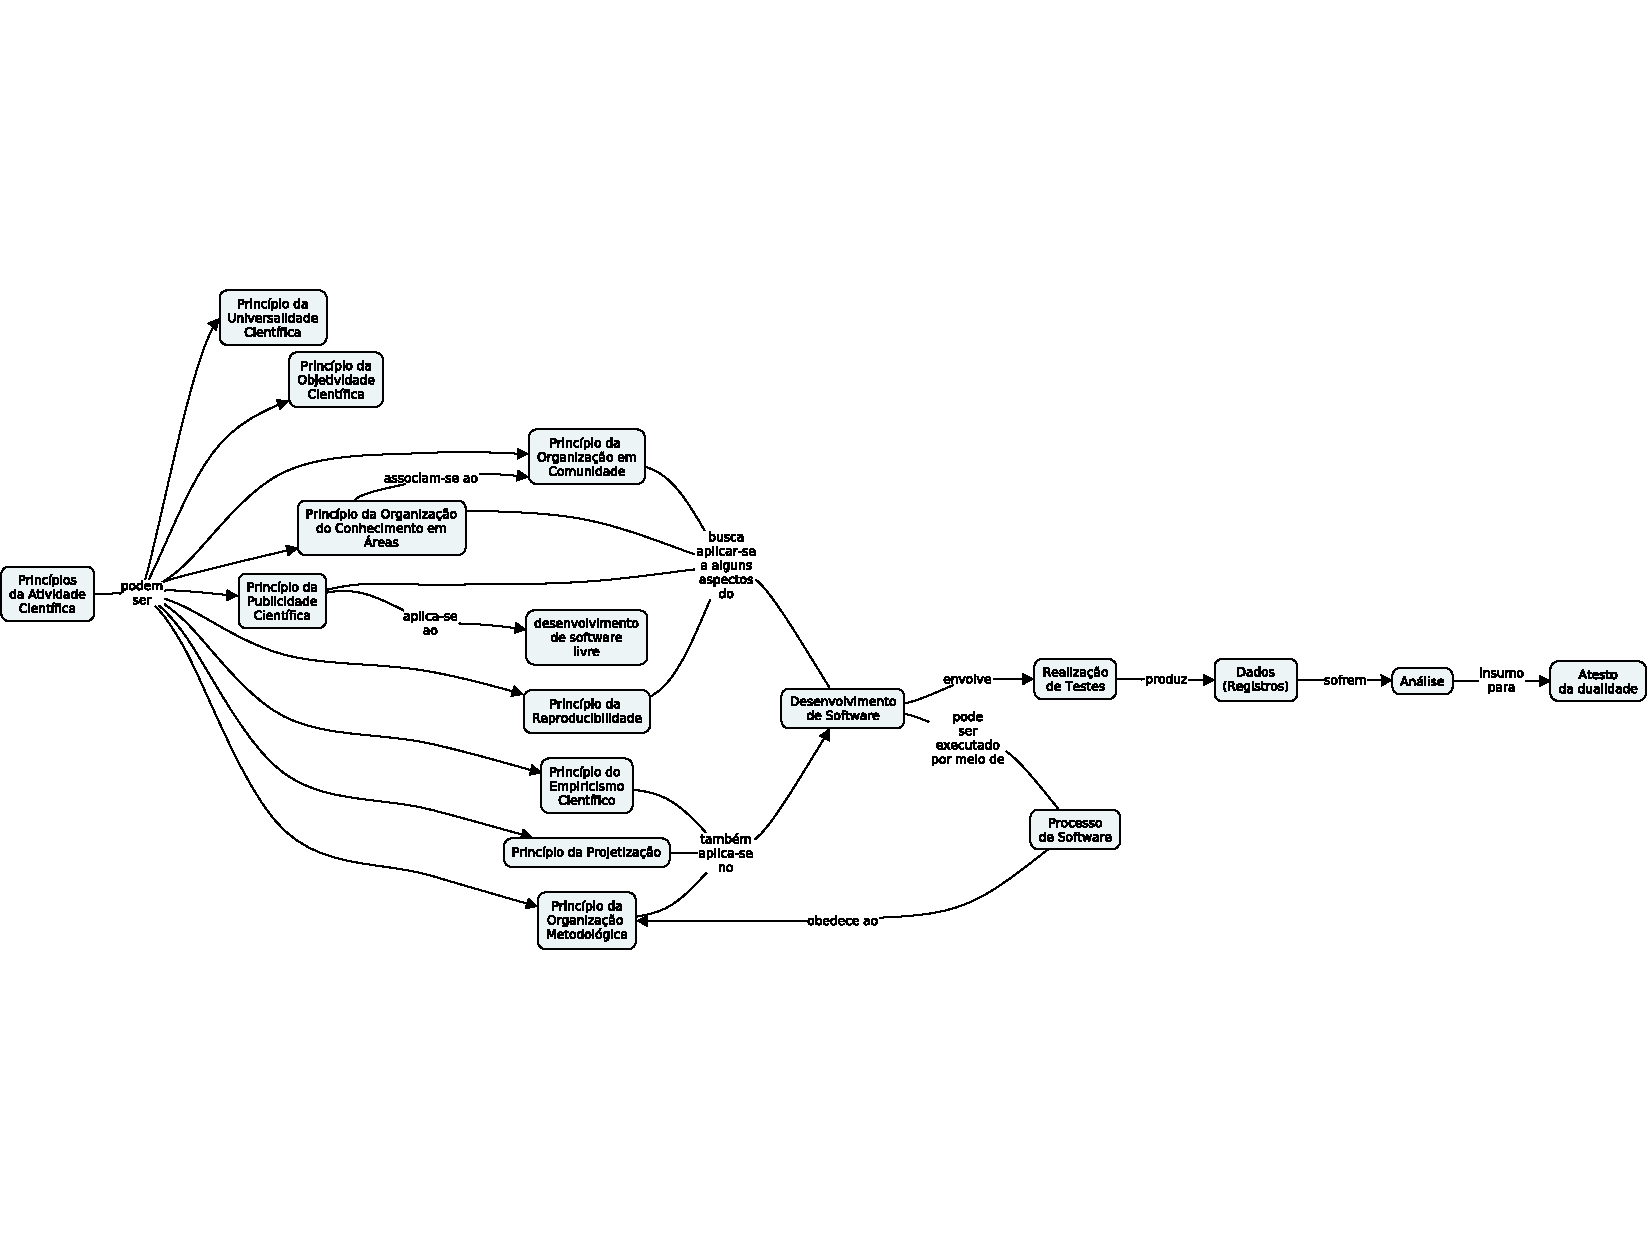
\includegraphics[page=1,angle=90,width=0.9\textwidth,height=0.9\textheight]{1-Introducao/aulas/Principios-da-atividade-cientifica.pdf}
    \caption{Quais os princípios da  atividade cientifica? como se relacionam com a atividade de desenvolvimento de software. Fonte: jhcf}
    \label{fig:principios:ativ:cientifica}
\end{figure}


	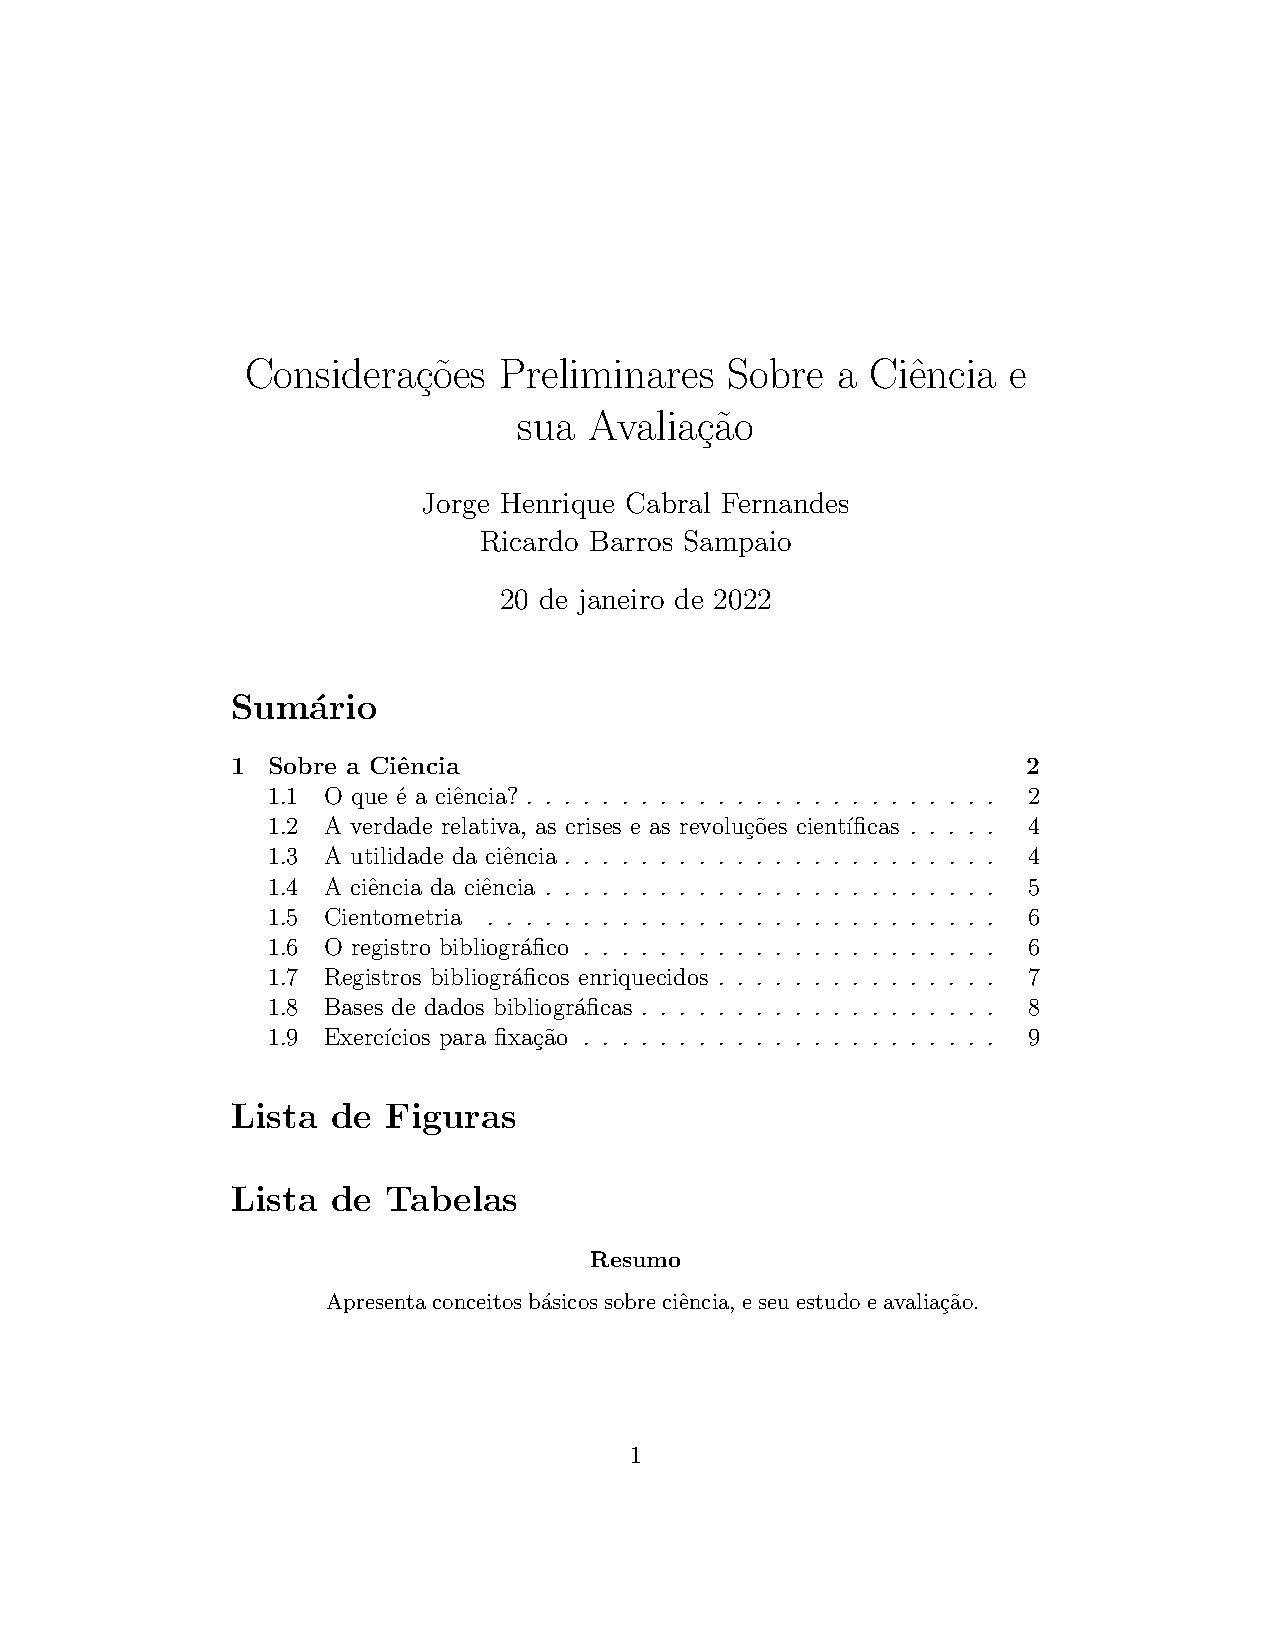
\includepdf[pages=-]{1-Introducao/aulas/Ciencia-e-sua-Avaliacao} 
    \chapter{Tarefa 9 - Teste Estatístico de Hipóteses e Estudos de Caso - Parte 2. 30 pontos\label{tarefa:teste:hipotese2:R}}

Antes de realizar essa tarefa, veja atentamente as instruções do capítulo anterior: "Conceitos Centrais em Estatística Inferencial".

Nessa tarefa você vai criar um novo capítulo, a partir do refinamento do capítulo anterior onde descreveu o seu laboratório com o teste para variáveis categóricas. Depois, vai fazer uma apresentação oral do seu capítulo em vídeo, conforme as orientações a seguir.
%como no modelo da seção \ref{tarefa:teste:hipotese:R:jhcf}, contendo um %texto com as seguintes características:

\section{Revise o texto da tarefa anterior}

Revise cuidadosamente todo o texto da tarefa anteriormente realizada, para que nada do que foi solicitado fique ausente.

\section{Teste do Chi-Quadrado} 

O teste do Chi-Quadrado permite explorar a chance de associação não aleatória entre dados categóricos, na forma de uma tabela crosstable. Crie uma seção que explora, declara e verifica hipóteses usando esse tipo de teste, com os dados de seu experimento. Adote como exemplo o código da listagem a seguir.

 \lstinputlisting[numbers=left,language={R},basicstyle=\tiny\ttfamily,caption={Realizando um teste de chi quadrado com amostras de um experimento},label={code:jhf:X2testCode}]{4-Computacao-Experimental/tarefas/T9-Teste-Hipoteses2/chi-square.R}
 
\section{Estudo de Caso}

Adote a abordagem de estudo de caso, para analise e descrição da evolução de um único experimento executado no seu simulador, desde o início até o alcance de estabilidade do fenômeno. Ao final, caracterize o experimento como sendo um caso típico ou de situação extrema, conforme as análises anteriores.

Crie uma seção chamada Estudo de Caso, para conter sua descrição.
Use pelo menos 250 palavras para essa seção.  

\section{Ética}

Vídeos e site:
\begin{description}
    \item [\url{https://www.youtube.com/watch?v=thbKYoLN1Ek}]
    \item [\url{https://www.youtube.com/watch?v=p6Ls45MVETk}]
    \item [Plataforma Brasil] \url{https://plataformabrasil.saude.gov.br/login.jsf}
\end{description}

Conforme os seus conhecimento de ética na realização de experimentos, discorra sobre as implicações éticas da realização de experimentos no mundo real, relativos ao fenômeno investigado.
Use pelo menos 250 palavras para essa seção.  

\section{Apresentação em Vídeo}
 
 Faça uma gravação da apresentação em vídeo do seu capítulo, nas reuniões de nomes "Apresentações em Vídeo A", "Apresentações em Vídeo B" ou "Apresentações em Vídeo C", disponíveis no ambiente Teams da disciplina, contendo os seguintes aspectos:
 \begin{description}
     \item [Seu rosto] Inicie apresentando o seu rosto, seu nome e dizendo o que contém o vídeo: "Uma apresentação do seu laboratório";
     \item [Texto] Compartilhe o texto do seu capítulo, para conduzir o restante da apresentação;
     \item [Execução do simulador] Apresente o seu simulador em execução interativa, mostrando como ele pode ser usado de forma prática; e
     \item [Hipóteses e resultados dos testes] Apresente os testes de hipóteses significativamente estatísticas que você fez, e interprete os resultados. 
 \end{description}
Não esqueça de gravar seu vídeo.

O seu vídeo deverá ter entre 5 e 15 minutos de duração.


% \begin{enumerate}
%     \item [Seção Introdução] Revise a apresentação das seções, já que o seu capítulo agora ficou mais extenso; 
%     \item [Seção o ``O Laboratório'']
%     \begin{description}
%     \item [Variáveis independentes ou de controle]
%     Registre e apresente, necessariamente, uma ou mais figuras com a interface  simulador, onde estão presentes as variáveis que podem ser independentes ajustadas, bem como as variáveis dependentes. Para cada variável independente ou de controle, informe se ela é do tipo (\url{https://rcompanion.org/handbook/C_01.html}):
%     \begin{description}
%     \item [nominal] ``Variáveis nominais são aquelas cujos níveis são rótulos ou descrições e que não podem ser ordenados. Exemplos de variáveis nominais são sexo, escola e perguntas sim/não. Eles também são chamados de variáveis “categóricas nominais” ou “qualitativas”, e os níveis de uma variável são às vezes chamados de “classes” ou “grupos”''
%     \item [ordinal] ``As variáveis ordinais são aquelas cujos valores podem ser ordenados ou classificados em ordem lógica, mas o intervalo entre os níveis das variáveis não é necessariamente conhecido. Medidas subjetivas são frequentemente variáveis ordinais. Um exemplo seria fazer com que as pessoas classificassem quatro itens por preferência em ordem de um a quatro. Um exemplo diferente seria fazer com que as pessoas avaliassem vários itens com base em uma escala de classificação Likert: “Em uma escala de um a cinco, você concorda ou discorda dessa afirmação?”. Um terceiro exemplo é o nível de escolaridade para adultos, considerando, por exemplo, “menor que o ensino médio”, “ensino médio”, “superior”, etc.''
%     \item [intervalar] ``As variáveis de intervalo ou razão são aquelas que representam valores medidos ou contados: idade, altura, peso, número de alunos. Sabe-se que o intervalo entre os números é igual: o intervalo entre um quilograma e dois quilogramas é o mesmo que entre três quilogramas e quatro quilogramas.
%  Os dados de intervalo/proporção também são chamados de dados “quantitativos”.

%     \item [intervalar discreta e contínua] 
% "Variáveis intervalares discretas e contínuas, são uma divisão de dados de intervalo ou razão. Nas intervalares discretas, os valores são necessariamente números inteiros ou outros valores discretos, como população ou contagens de itens. As variáveis intervalares contínuas podem assumir qualquer valor dentro de um intervalo e, portanto, podem ser expressas como decimais. Muitas vezes são quantidades medidas. Por exemplo, em teoria, um peso pode ser medido como 1 kg, 1,01 kg ou 1,009 kg e assim por diante. A idade também pode ser considerada uma variável contínua, embora muitas vezes a tratemos como uma variável discreta, arredondando-a para o aniversário mais recente."
%     \end{description}
%     \item [Código do Simulador]
%     Apresente, no código do seu simulador, as partes que introduzem a aleatoriedade dos fenômenos de interação entre os agentes, e argumente de que forma essa aleatoriedade no código contribui para que as amostras do fenômeno simulado também sejam aleatórias. 
%     \end{description}
    
%     \begin{description}
%         \item [Apresentação das Amostras] Nessa seção, refine o que antes era apenas a apresentação das "Variáveis Dependentes e Independentes", nos seguintes termos: 
%         Descreva cada uma das colunas da planilha de amostras de experimentos por você coletadas, informando:
%         \begin{itemize}
%             \item O nome da variável;
%             \item O que significa a variável;
%             \item Se a variável é para uso interno do simulador, variável de controle no experimento, variável independente ou variável dependente;
%             \item As faixas de valores ou categorias dos registros obtidos, para fins de interpretação dos números (ex: Se umidade = 0, o que isso significa? Se umidade = 1, o que significa?;
%         \end{itemize}
        
%         \item [Primeira Declaração Formal de Hipóteses] Revise o texto da sua primeira declaração formal de hipóteses.
        
%         \item [Aplicação do Teste t] 
%         Revise o texto de aplicação do teste t.
        
%         \item [Segunda Declaração Formal de Hipóteses] Revise o texto da sua segunda declaração formal de hipóteses.
    
%         \item [Aplicação do teste de regressão linear] Revise o texto da aplicação do teste de regressão linear.
        
%         \item [Teste do Chi-Quadrado] 
%         Revise o texto da sua primeira declaração formal de hipóteses.
        
%         Supondo que foi feita a escolha inicial do teste t de Student, para comparar médias entre duas amostras (conjunto de registros) de variável dependente, que foram obtidas a partir de estímulos com diferentes valores para pelo menos uma variável independente, faça uma declaração de hipóteses nula e alternativa para o seu teste. Aplique corretamente os conceitos de hipóteses nula e alternativa, conforme o vídeo sobre Inferência Estatística.
%         \item [Aplicação do Teste t] Use as instruções em \url{https://stat.ethz.ch/R-manual/R-devel/library/stats/html/t.test.html}, e com base no vídeo sobre teste t (\url{https://www.youtube.com/watch?v=AgDC9yoopUA}), apresente duas diferentes execuções do teste, comparando diferentes amostras. Apresente, usando lstlistings, todo o código R usado, os resultados apresentados no Console do R, e sua interpretação dos resultados. Informe sobre a comprovação ou rejeição da hipótese nula;
%         \item [Segunda Declaração Formal de Hipóteses] Supondo que agora vais fazer uma análise de regressão linear, com as mesmas amostras, veja o vídeo e o texto sobre regressão linear em R:
%         \begin{itemize}
%             \item \url{https://www.youtube.com/watch?v=u1cc1r_Y7M0}; e
%             \item \url{https://www.r-tutor.com/elementary-statistics/simple-linear-regression/significance-test-linear-regression}.
%         \end{itemize}
%         Com base nos vídeos, faça uma declaração de hipóteses nula e alternativa para o seu teste, que estabeleça possível relação linear entre uma variável independente e uma dependente. Aplique corretamente os conceitos de hipóteses nula e alternativa.
%         \item [Aplicação do teste de regressão linear] Apresente duas diferentes execuções do teste, comparando diferentes amostras por meio de regressão linear. Apresente todo o código R dos comandos e dos resultados apresentados no Console do R, e sua interpretação dos resultados, sobre a comprovação ou não da hipótese nula;
%         \item [Conclusões] Apresente suas conclusões sobre os testes realizados.
%     \end{description}
%  \end{enumerate}
    
%\chapter{Manipulação de Variáveis em Simulações}

Neste capítulo você aprenderá a projetar e codificar a manipulação de variáveis no seu modelo de simulação, que posteriormente serão consideradas variáveis independentes ou de controle de um experimento.



    
    \chapter{Tarefa 9 - Teste Estatístico de Hipóteses e Estudos de Caso - Parte 2. 30 pontos\label{tarefa:teste:hipotese2:R}}

Antes de realizar essa tarefa, veja atentamente as instruções do capítulo anterior: "Conceitos Centrais em Estatística Inferencial".

Nessa tarefa você vai criar um novo capítulo, a partir do refinamento do capítulo anterior onde descreveu o seu laboratório com o teste para variáveis categóricas. Depois, vai fazer uma apresentação oral do seu capítulo em vídeo, conforme as orientações a seguir.
%como no modelo da seção \ref{tarefa:teste:hipotese:R:jhcf}, contendo um %texto com as seguintes características:

\section{Revise o texto da tarefa anterior}

Revise cuidadosamente todo o texto da tarefa anteriormente realizada, para que nada do que foi solicitado fique ausente.

\section{Teste do Chi-Quadrado} 

O teste do Chi-Quadrado permite explorar a chance de associação não aleatória entre dados categóricos, na forma de uma tabela crosstable. Crie uma seção que explora, declara e verifica hipóteses usando esse tipo de teste, com os dados de seu experimento. Adote como exemplo o código da listagem a seguir.

 \lstinputlisting[numbers=left,language={R},basicstyle=\tiny\ttfamily,caption={Realizando um teste de chi quadrado com amostras de um experimento},label={code:jhf:X2testCode}]{4-Computacao-Experimental/tarefas/T9-Teste-Hipoteses2/chi-square.R}
 
\section{Estudo de Caso}

Adote a abordagem de estudo de caso, para analise e descrição da evolução de um único experimento executado no seu simulador, desde o início até o alcance de estabilidade do fenômeno. Ao final, caracterize o experimento como sendo um caso típico ou de situação extrema, conforme as análises anteriores.

Crie uma seção chamada Estudo de Caso, para conter sua descrição.
Use pelo menos 250 palavras para essa seção.  

\section{Ética}

Vídeos e site:
\begin{description}
    \item [\url{https://www.youtube.com/watch?v=thbKYoLN1Ek}]
    \item [\url{https://www.youtube.com/watch?v=p6Ls45MVETk}]
    \item [Plataforma Brasil] \url{https://plataformabrasil.saude.gov.br/login.jsf}
\end{description}

Conforme os seus conhecimento de ética na realização de experimentos, discorra sobre as implicações éticas da realização de experimentos no mundo real, relativos ao fenômeno investigado.
Use pelo menos 250 palavras para essa seção.  

\section{Apresentação em Vídeo}
 
 Faça uma gravação da apresentação em vídeo do seu capítulo, nas reuniões de nomes "Apresentações em Vídeo A", "Apresentações em Vídeo B" ou "Apresentações em Vídeo C", disponíveis no ambiente Teams da disciplina, contendo os seguintes aspectos:
 \begin{description}
     \item [Seu rosto] Inicie apresentando o seu rosto, seu nome e dizendo o que contém o vídeo: "Uma apresentação do seu laboratório";
     \item [Texto] Compartilhe o texto do seu capítulo, para conduzir o restante da apresentação;
     \item [Execução do simulador] Apresente o seu simulador em execução interativa, mostrando como ele pode ser usado de forma prática; e
     \item [Hipóteses e resultados dos testes] Apresente os testes de hipóteses significativamente estatísticas que você fez, e interprete os resultados. 
 \end{description}
Não esqueça de gravar seu vídeo.

O seu vídeo deverá ter entre 5 e 15 minutos de duração.


% \begin{enumerate}
%     \item [Seção Introdução] Revise a apresentação das seções, já que o seu capítulo agora ficou mais extenso; 
%     \item [Seção o ``O Laboratório'']
%     \begin{description}
%     \item [Variáveis independentes ou de controle]
%     Registre e apresente, necessariamente, uma ou mais figuras com a interface  simulador, onde estão presentes as variáveis que podem ser independentes ajustadas, bem como as variáveis dependentes. Para cada variável independente ou de controle, informe se ela é do tipo (\url{https://rcompanion.org/handbook/C_01.html}):
%     \begin{description}
%     \item [nominal] ``Variáveis nominais são aquelas cujos níveis são rótulos ou descrições e que não podem ser ordenados. Exemplos de variáveis nominais são sexo, escola e perguntas sim/não. Eles também são chamados de variáveis “categóricas nominais” ou “qualitativas”, e os níveis de uma variável são às vezes chamados de “classes” ou “grupos”''
%     \item [ordinal] ``As variáveis ordinais são aquelas cujos valores podem ser ordenados ou classificados em ordem lógica, mas o intervalo entre os níveis das variáveis não é necessariamente conhecido. Medidas subjetivas são frequentemente variáveis ordinais. Um exemplo seria fazer com que as pessoas classificassem quatro itens por preferência em ordem de um a quatro. Um exemplo diferente seria fazer com que as pessoas avaliassem vários itens com base em uma escala de classificação Likert: “Em uma escala de um a cinco, você concorda ou discorda dessa afirmação?”. Um terceiro exemplo é o nível de escolaridade para adultos, considerando, por exemplo, “menor que o ensino médio”, “ensino médio”, “superior”, etc.''
%     \item [intervalar] ``As variáveis de intervalo ou razão são aquelas que representam valores medidos ou contados: idade, altura, peso, número de alunos. Sabe-se que o intervalo entre os números é igual: o intervalo entre um quilograma e dois quilogramas é o mesmo que entre três quilogramas e quatro quilogramas.
%  Os dados de intervalo/proporção também são chamados de dados “quantitativos”.

%     \item [intervalar discreta e contínua] 
% "Variáveis intervalares discretas e contínuas, são uma divisão de dados de intervalo ou razão. Nas intervalares discretas, os valores são necessariamente números inteiros ou outros valores discretos, como população ou contagens de itens. As variáveis intervalares contínuas podem assumir qualquer valor dentro de um intervalo e, portanto, podem ser expressas como decimais. Muitas vezes são quantidades medidas. Por exemplo, em teoria, um peso pode ser medido como 1 kg, 1,01 kg ou 1,009 kg e assim por diante. A idade também pode ser considerada uma variável contínua, embora muitas vezes a tratemos como uma variável discreta, arredondando-a para o aniversário mais recente."
%     \end{description}
%     \item [Código do Simulador]
%     Apresente, no código do seu simulador, as partes que introduzem a aleatoriedade dos fenômenos de interação entre os agentes, e argumente de que forma essa aleatoriedade no código contribui para que as amostras do fenômeno simulado também sejam aleatórias. 
%     \end{description}
    
%     \begin{description}
%         \item [Apresentação das Amostras] Nessa seção, refine o que antes era apenas a apresentação das "Variáveis Dependentes e Independentes", nos seguintes termos: 
%         Descreva cada uma das colunas da planilha de amostras de experimentos por você coletadas, informando:
%         \begin{itemize}
%             \item O nome da variável;
%             \item O que significa a variável;
%             \item Se a variável é para uso interno do simulador, variável de controle no experimento, variável independente ou variável dependente;
%             \item As faixas de valores ou categorias dos registros obtidos, para fins de interpretação dos números (ex: Se umidade = 0, o que isso significa? Se umidade = 1, o que significa?;
%         \end{itemize}
        
%         \item [Primeira Declaração Formal de Hipóteses] Revise o texto da sua primeira declaração formal de hipóteses.
        
%         \item [Aplicação do Teste t] 
%         Revise o texto de aplicação do teste t.
        
%         \item [Segunda Declaração Formal de Hipóteses] Revise o texto da sua segunda declaração formal de hipóteses.
    
%         \item [Aplicação do teste de regressão linear] Revise o texto da aplicação do teste de regressão linear.
        
%         \item [Teste do Chi-Quadrado] 
%         Revise o texto da sua primeira declaração formal de hipóteses.
        
%         Supondo que foi feita a escolha inicial do teste t de Student, para comparar médias entre duas amostras (conjunto de registros) de variável dependente, que foram obtidas a partir de estímulos com diferentes valores para pelo menos uma variável independente, faça uma declaração de hipóteses nula e alternativa para o seu teste. Aplique corretamente os conceitos de hipóteses nula e alternativa, conforme o vídeo sobre Inferência Estatística.
%         \item [Aplicação do Teste t] Use as instruções em \url{https://stat.ethz.ch/R-manual/R-devel/library/stats/html/t.test.html}, e com base no vídeo sobre teste t (\url{https://www.youtube.com/watch?v=AgDC9yoopUA}), apresente duas diferentes execuções do teste, comparando diferentes amostras. Apresente, usando lstlistings, todo o código R usado, os resultados apresentados no Console do R, e sua interpretação dos resultados. Informe sobre a comprovação ou rejeição da hipótese nula;
%         \item [Segunda Declaração Formal de Hipóteses] Supondo que agora vais fazer uma análise de regressão linear, com as mesmas amostras, veja o vídeo e o texto sobre regressão linear em R:
%         \begin{itemize}
%             \item \url{https://www.youtube.com/watch?v=u1cc1r_Y7M0}; e
%             \item \url{https://www.r-tutor.com/elementary-statistics/simple-linear-regression/significance-test-linear-regression}.
%         \end{itemize}
%         Com base nos vídeos, faça uma declaração de hipóteses nula e alternativa para o seu teste, que estabeleça possível relação linear entre uma variável independente e uma dependente. Aplique corretamente os conceitos de hipóteses nula e alternativa.
%         \item [Aplicação do teste de regressão linear] Apresente duas diferentes execuções do teste, comparando diferentes amostras por meio de regressão linear. Apresente todo o código R dos comandos e dos resultados apresentados no Console do R, e sua interpretação dos resultados, sobre a comprovação ou não da hipótese nula;
%         \item [Conclusões] Apresente suas conclusões sobre os testes realizados.
%     \end{description}
%  \end{enumerate}
    
%\chapter{Manipulação de Variáveis em Simulações}

Neste capítulo você aprenderá a projetar e codificar a manipulação de variáveis no seu modelo de simulação, que posteriormente serão consideradas variáveis independentes ou de controle de um experimento.




    \chapter{Manipulação de Variáveis em Simulações}

Neste capítulo você aprenderá a projetar e codificar a manipulação de variáveis no seu modelo de simulação, que posteriormente serão consideradas variáveis independentes ou de controle de um experimento.



\part{Pesquisa Bibliométrica\label{part:biblio}}

    \chapter{Manipulação de Variáveis em Simulações}

Neste capítulo você aprenderá a projetar e codificar a manipulação de variáveis no seu modelo de simulação, que posteriormente serão consideradas variáveis independentes ou de controle de um experimento.



    \chapter{Manipulação de Variáveis em Simulações}

Neste capítulo você aprenderá a projetar e codificar a manipulação de variáveis no seu modelo de simulação, que posteriormente serão consideradas variáveis independentes ou de controle de um experimento.



    \chapter{Tarefa 9 - Teste Estatístico de Hipóteses e Estudos de Caso - Parte 2. 30 pontos\label{tarefa:teste:hipotese2:R}}

Antes de realizar essa tarefa, veja atentamente as instruções do capítulo anterior: "Conceitos Centrais em Estatística Inferencial".

Nessa tarefa você vai criar um novo capítulo, a partir do refinamento do capítulo anterior onde descreveu o seu laboratório com o teste para variáveis categóricas. Depois, vai fazer uma apresentação oral do seu capítulo em vídeo, conforme as orientações a seguir.
%como no modelo da seção \ref{tarefa:teste:hipotese:R:jhcf}, contendo um %texto com as seguintes características:

\section{Revise o texto da tarefa anterior}

Revise cuidadosamente todo o texto da tarefa anteriormente realizada, para que nada do que foi solicitado fique ausente.

\section{Teste do Chi-Quadrado} 

O teste do Chi-Quadrado permite explorar a chance de associação não aleatória entre dados categóricos, na forma de uma tabela crosstable. Crie uma seção que explora, declara e verifica hipóteses usando esse tipo de teste, com os dados de seu experimento. Adote como exemplo o código da listagem a seguir.

 \lstinputlisting[numbers=left,language={R},basicstyle=\tiny\ttfamily,caption={Realizando um teste de chi quadrado com amostras de um experimento},label={code:jhf:X2testCode}]{4-Computacao-Experimental/tarefas/T9-Teste-Hipoteses2/chi-square.R}
 
\section{Estudo de Caso}

Adote a abordagem de estudo de caso, para analise e descrição da evolução de um único experimento executado no seu simulador, desde o início até o alcance de estabilidade do fenômeno. Ao final, caracterize o experimento como sendo um caso típico ou de situação extrema, conforme as análises anteriores.

Crie uma seção chamada Estudo de Caso, para conter sua descrição.
Use pelo menos 250 palavras para essa seção.  

\section{Ética}

Vídeos e site:
\begin{description}
    \item [\url{https://www.youtube.com/watch?v=thbKYoLN1Ek}]
    \item [\url{https://www.youtube.com/watch?v=p6Ls45MVETk}]
    \item [Plataforma Brasil] \url{https://plataformabrasil.saude.gov.br/login.jsf}
\end{description}

Conforme os seus conhecimento de ética na realização de experimentos, discorra sobre as implicações éticas da realização de experimentos no mundo real, relativos ao fenômeno investigado.
Use pelo menos 250 palavras para essa seção.  

\section{Apresentação em Vídeo}
 
 Faça uma gravação da apresentação em vídeo do seu capítulo, nas reuniões de nomes "Apresentações em Vídeo A", "Apresentações em Vídeo B" ou "Apresentações em Vídeo C", disponíveis no ambiente Teams da disciplina, contendo os seguintes aspectos:
 \begin{description}
     \item [Seu rosto] Inicie apresentando o seu rosto, seu nome e dizendo o que contém o vídeo: "Uma apresentação do seu laboratório";
     \item [Texto] Compartilhe o texto do seu capítulo, para conduzir o restante da apresentação;
     \item [Execução do simulador] Apresente o seu simulador em execução interativa, mostrando como ele pode ser usado de forma prática; e
     \item [Hipóteses e resultados dos testes] Apresente os testes de hipóteses significativamente estatísticas que você fez, e interprete os resultados. 
 \end{description}
Não esqueça de gravar seu vídeo.

O seu vídeo deverá ter entre 5 e 15 minutos de duração.


% \begin{enumerate}
%     \item [Seção Introdução] Revise a apresentação das seções, já que o seu capítulo agora ficou mais extenso; 
%     \item [Seção o ``O Laboratório'']
%     \begin{description}
%     \item [Variáveis independentes ou de controle]
%     Registre e apresente, necessariamente, uma ou mais figuras com a interface  simulador, onde estão presentes as variáveis que podem ser independentes ajustadas, bem como as variáveis dependentes. Para cada variável independente ou de controle, informe se ela é do tipo (\url{https://rcompanion.org/handbook/C_01.html}):
%     \begin{description}
%     \item [nominal] ``Variáveis nominais são aquelas cujos níveis são rótulos ou descrições e que não podem ser ordenados. Exemplos de variáveis nominais são sexo, escola e perguntas sim/não. Eles também são chamados de variáveis “categóricas nominais” ou “qualitativas”, e os níveis de uma variável são às vezes chamados de “classes” ou “grupos”''
%     \item [ordinal] ``As variáveis ordinais são aquelas cujos valores podem ser ordenados ou classificados em ordem lógica, mas o intervalo entre os níveis das variáveis não é necessariamente conhecido. Medidas subjetivas são frequentemente variáveis ordinais. Um exemplo seria fazer com que as pessoas classificassem quatro itens por preferência em ordem de um a quatro. Um exemplo diferente seria fazer com que as pessoas avaliassem vários itens com base em uma escala de classificação Likert: “Em uma escala de um a cinco, você concorda ou discorda dessa afirmação?”. Um terceiro exemplo é o nível de escolaridade para adultos, considerando, por exemplo, “menor que o ensino médio”, “ensino médio”, “superior”, etc.''
%     \item [intervalar] ``As variáveis de intervalo ou razão são aquelas que representam valores medidos ou contados: idade, altura, peso, número de alunos. Sabe-se que o intervalo entre os números é igual: o intervalo entre um quilograma e dois quilogramas é o mesmo que entre três quilogramas e quatro quilogramas.
%  Os dados de intervalo/proporção também são chamados de dados “quantitativos”.

%     \item [intervalar discreta e contínua] 
% "Variáveis intervalares discretas e contínuas, são uma divisão de dados de intervalo ou razão. Nas intervalares discretas, os valores são necessariamente números inteiros ou outros valores discretos, como população ou contagens de itens. As variáveis intervalares contínuas podem assumir qualquer valor dentro de um intervalo e, portanto, podem ser expressas como decimais. Muitas vezes são quantidades medidas. Por exemplo, em teoria, um peso pode ser medido como 1 kg, 1,01 kg ou 1,009 kg e assim por diante. A idade também pode ser considerada uma variável contínua, embora muitas vezes a tratemos como uma variável discreta, arredondando-a para o aniversário mais recente."
%     \end{description}
%     \item [Código do Simulador]
%     Apresente, no código do seu simulador, as partes que introduzem a aleatoriedade dos fenômenos de interação entre os agentes, e argumente de que forma essa aleatoriedade no código contribui para que as amostras do fenômeno simulado também sejam aleatórias. 
%     \end{description}
    
%     \begin{description}
%         \item [Apresentação das Amostras] Nessa seção, refine o que antes era apenas a apresentação das "Variáveis Dependentes e Independentes", nos seguintes termos: 
%         Descreva cada uma das colunas da planilha de amostras de experimentos por você coletadas, informando:
%         \begin{itemize}
%             \item O nome da variável;
%             \item O que significa a variável;
%             \item Se a variável é para uso interno do simulador, variável de controle no experimento, variável independente ou variável dependente;
%             \item As faixas de valores ou categorias dos registros obtidos, para fins de interpretação dos números (ex: Se umidade = 0, o que isso significa? Se umidade = 1, o que significa?;
%         \end{itemize}
        
%         \item [Primeira Declaração Formal de Hipóteses] Revise o texto da sua primeira declaração formal de hipóteses.
        
%         \item [Aplicação do Teste t] 
%         Revise o texto de aplicação do teste t.
        
%         \item [Segunda Declaração Formal de Hipóteses] Revise o texto da sua segunda declaração formal de hipóteses.
    
%         \item [Aplicação do teste de regressão linear] Revise o texto da aplicação do teste de regressão linear.
        
%         \item [Teste do Chi-Quadrado] 
%         Revise o texto da sua primeira declaração formal de hipóteses.
        
%         Supondo que foi feita a escolha inicial do teste t de Student, para comparar médias entre duas amostras (conjunto de registros) de variável dependente, que foram obtidas a partir de estímulos com diferentes valores para pelo menos uma variável independente, faça uma declaração de hipóteses nula e alternativa para o seu teste. Aplique corretamente os conceitos de hipóteses nula e alternativa, conforme o vídeo sobre Inferência Estatística.
%         \item [Aplicação do Teste t] Use as instruções em \url{https://stat.ethz.ch/R-manual/R-devel/library/stats/html/t.test.html}, e com base no vídeo sobre teste t (\url{https://www.youtube.com/watch?v=AgDC9yoopUA}), apresente duas diferentes execuções do teste, comparando diferentes amostras. Apresente, usando lstlistings, todo o código R usado, os resultados apresentados no Console do R, e sua interpretação dos resultados. Informe sobre a comprovação ou rejeição da hipótese nula;
%         \item [Segunda Declaração Formal de Hipóteses] Supondo que agora vais fazer uma análise de regressão linear, com as mesmas amostras, veja o vídeo e o texto sobre regressão linear em R:
%         \begin{itemize}
%             \item \url{https://www.youtube.com/watch?v=u1cc1r_Y7M0}; e
%             \item \url{https://www.r-tutor.com/elementary-statistics/simple-linear-regression/significance-test-linear-regression}.
%         \end{itemize}
%         Com base nos vídeos, faça uma declaração de hipóteses nula e alternativa para o seu teste, que estabeleça possível relação linear entre uma variável independente e uma dependente. Aplique corretamente os conceitos de hipóteses nula e alternativa.
%         \item [Aplicação do teste de regressão linear] Apresente duas diferentes execuções do teste, comparando diferentes amostras por meio de regressão linear. Apresente todo o código R dos comandos e dos resultados apresentados no Console do R, e sua interpretação dos resultados, sobre a comprovação ou não da hipótese nula;
%         \item [Conclusões] Apresente suas conclusões sobre os testes realizados.
%     \end{description}
%  \end{enumerate}
    
%\chapter{Manipulação de Variáveis em Simulações}

Neste capítulo você aprenderá a projetar e codificar a manipulação de variáveis no seu modelo de simulação, que posteriormente serão consideradas variáveis independentes ou de controle de um experimento.




\chapter{Tarefas T4 entregues pelos Estudantes}

    \chapter{Manipulação de Variáveis em Simulações}

Neste capítulo você aprenderá a projetar e codificar a manipulação de variáveis no seu modelo de simulação, que posteriormente serão consideradas variáveis independentes ou de controle de um experimento.



\part{Simulação Computacional\label{part:simulacao}}

    \chapter{Manipulação de Variáveis em Simulações}

Neste capítulo você aprenderá a projetar e codificar a manipulação de variáveis no seu modelo de simulação, que posteriormente serão consideradas variáveis independentes ou de controle de um experimento.



    \chapter{Tarefa 9 - Teste Estatístico de Hipóteses e Estudos de Caso - Parte 2. 30 pontos\label{tarefa:teste:hipotese2:R}}

Antes de realizar essa tarefa, veja atentamente as instruções do capítulo anterior: "Conceitos Centrais em Estatística Inferencial".

Nessa tarefa você vai criar um novo capítulo, a partir do refinamento do capítulo anterior onde descreveu o seu laboratório com o teste para variáveis categóricas. Depois, vai fazer uma apresentação oral do seu capítulo em vídeo, conforme as orientações a seguir.
%como no modelo da seção \ref{tarefa:teste:hipotese:R:jhcf}, contendo um %texto com as seguintes características:

\section{Revise o texto da tarefa anterior}

Revise cuidadosamente todo o texto da tarefa anteriormente realizada, para que nada do que foi solicitado fique ausente.

\section{Teste do Chi-Quadrado} 

O teste do Chi-Quadrado permite explorar a chance de associação não aleatória entre dados categóricos, na forma de uma tabela crosstable. Crie uma seção que explora, declara e verifica hipóteses usando esse tipo de teste, com os dados de seu experimento. Adote como exemplo o código da listagem a seguir.

 \lstinputlisting[numbers=left,language={R},basicstyle=\tiny\ttfamily,caption={Realizando um teste de chi quadrado com amostras de um experimento},label={code:jhf:X2testCode}]{4-Computacao-Experimental/tarefas/T9-Teste-Hipoteses2/chi-square.R}
 
\section{Estudo de Caso}

Adote a abordagem de estudo de caso, para analise e descrição da evolução de um único experimento executado no seu simulador, desde o início até o alcance de estabilidade do fenômeno. Ao final, caracterize o experimento como sendo um caso típico ou de situação extrema, conforme as análises anteriores.

Crie uma seção chamada Estudo de Caso, para conter sua descrição.
Use pelo menos 250 palavras para essa seção.  

\section{Ética}

Vídeos e site:
\begin{description}
    \item [\url{https://www.youtube.com/watch?v=thbKYoLN1Ek}]
    \item [\url{https://www.youtube.com/watch?v=p6Ls45MVETk}]
    \item [Plataforma Brasil] \url{https://plataformabrasil.saude.gov.br/login.jsf}
\end{description}

Conforme os seus conhecimento de ética na realização de experimentos, discorra sobre as implicações éticas da realização de experimentos no mundo real, relativos ao fenômeno investigado.
Use pelo menos 250 palavras para essa seção.  

\section{Apresentação em Vídeo}
 
 Faça uma gravação da apresentação em vídeo do seu capítulo, nas reuniões de nomes "Apresentações em Vídeo A", "Apresentações em Vídeo B" ou "Apresentações em Vídeo C", disponíveis no ambiente Teams da disciplina, contendo os seguintes aspectos:
 \begin{description}
     \item [Seu rosto] Inicie apresentando o seu rosto, seu nome e dizendo o que contém o vídeo: "Uma apresentação do seu laboratório";
     \item [Texto] Compartilhe o texto do seu capítulo, para conduzir o restante da apresentação;
     \item [Execução do simulador] Apresente o seu simulador em execução interativa, mostrando como ele pode ser usado de forma prática; e
     \item [Hipóteses e resultados dos testes] Apresente os testes de hipóteses significativamente estatísticas que você fez, e interprete os resultados. 
 \end{description}
Não esqueça de gravar seu vídeo.

O seu vídeo deverá ter entre 5 e 15 minutos de duração.


% \begin{enumerate}
%     \item [Seção Introdução] Revise a apresentação das seções, já que o seu capítulo agora ficou mais extenso; 
%     \item [Seção o ``O Laboratório'']
%     \begin{description}
%     \item [Variáveis independentes ou de controle]
%     Registre e apresente, necessariamente, uma ou mais figuras com a interface  simulador, onde estão presentes as variáveis que podem ser independentes ajustadas, bem como as variáveis dependentes. Para cada variável independente ou de controle, informe se ela é do tipo (\url{https://rcompanion.org/handbook/C_01.html}):
%     \begin{description}
%     \item [nominal] ``Variáveis nominais são aquelas cujos níveis são rótulos ou descrições e que não podem ser ordenados. Exemplos de variáveis nominais são sexo, escola e perguntas sim/não. Eles também são chamados de variáveis “categóricas nominais” ou “qualitativas”, e os níveis de uma variável são às vezes chamados de “classes” ou “grupos”''
%     \item [ordinal] ``As variáveis ordinais são aquelas cujos valores podem ser ordenados ou classificados em ordem lógica, mas o intervalo entre os níveis das variáveis não é necessariamente conhecido. Medidas subjetivas são frequentemente variáveis ordinais. Um exemplo seria fazer com que as pessoas classificassem quatro itens por preferência em ordem de um a quatro. Um exemplo diferente seria fazer com que as pessoas avaliassem vários itens com base em uma escala de classificação Likert: “Em uma escala de um a cinco, você concorda ou discorda dessa afirmação?”. Um terceiro exemplo é o nível de escolaridade para adultos, considerando, por exemplo, “menor que o ensino médio”, “ensino médio”, “superior”, etc.''
%     \item [intervalar] ``As variáveis de intervalo ou razão são aquelas que representam valores medidos ou contados: idade, altura, peso, número de alunos. Sabe-se que o intervalo entre os números é igual: o intervalo entre um quilograma e dois quilogramas é o mesmo que entre três quilogramas e quatro quilogramas.
%  Os dados de intervalo/proporção também são chamados de dados “quantitativos”.

%     \item [intervalar discreta e contínua] 
% "Variáveis intervalares discretas e contínuas, são uma divisão de dados de intervalo ou razão. Nas intervalares discretas, os valores são necessariamente números inteiros ou outros valores discretos, como população ou contagens de itens. As variáveis intervalares contínuas podem assumir qualquer valor dentro de um intervalo e, portanto, podem ser expressas como decimais. Muitas vezes são quantidades medidas. Por exemplo, em teoria, um peso pode ser medido como 1 kg, 1,01 kg ou 1,009 kg e assim por diante. A idade também pode ser considerada uma variável contínua, embora muitas vezes a tratemos como uma variável discreta, arredondando-a para o aniversário mais recente."
%     \end{description}
%     \item [Código do Simulador]
%     Apresente, no código do seu simulador, as partes que introduzem a aleatoriedade dos fenômenos de interação entre os agentes, e argumente de que forma essa aleatoriedade no código contribui para que as amostras do fenômeno simulado também sejam aleatórias. 
%     \end{description}
    
%     \begin{description}
%         \item [Apresentação das Amostras] Nessa seção, refine o que antes era apenas a apresentação das "Variáveis Dependentes e Independentes", nos seguintes termos: 
%         Descreva cada uma das colunas da planilha de amostras de experimentos por você coletadas, informando:
%         \begin{itemize}
%             \item O nome da variável;
%             \item O que significa a variável;
%             \item Se a variável é para uso interno do simulador, variável de controle no experimento, variável independente ou variável dependente;
%             \item As faixas de valores ou categorias dos registros obtidos, para fins de interpretação dos números (ex: Se umidade = 0, o que isso significa? Se umidade = 1, o que significa?;
%         \end{itemize}
        
%         \item [Primeira Declaração Formal de Hipóteses] Revise o texto da sua primeira declaração formal de hipóteses.
        
%         \item [Aplicação do Teste t] 
%         Revise o texto de aplicação do teste t.
        
%         \item [Segunda Declaração Formal de Hipóteses] Revise o texto da sua segunda declaração formal de hipóteses.
    
%         \item [Aplicação do teste de regressão linear] Revise o texto da aplicação do teste de regressão linear.
        
%         \item [Teste do Chi-Quadrado] 
%         Revise o texto da sua primeira declaração formal de hipóteses.
        
%         Supondo que foi feita a escolha inicial do teste t de Student, para comparar médias entre duas amostras (conjunto de registros) de variável dependente, que foram obtidas a partir de estímulos com diferentes valores para pelo menos uma variável independente, faça uma declaração de hipóteses nula e alternativa para o seu teste. Aplique corretamente os conceitos de hipóteses nula e alternativa, conforme o vídeo sobre Inferência Estatística.
%         \item [Aplicação do Teste t] Use as instruções em \url{https://stat.ethz.ch/R-manual/R-devel/library/stats/html/t.test.html}, e com base no vídeo sobre teste t (\url{https://www.youtube.com/watch?v=AgDC9yoopUA}), apresente duas diferentes execuções do teste, comparando diferentes amostras. Apresente, usando lstlistings, todo o código R usado, os resultados apresentados no Console do R, e sua interpretação dos resultados. Informe sobre a comprovação ou rejeição da hipótese nula;
%         \item [Segunda Declaração Formal de Hipóteses] Supondo que agora vais fazer uma análise de regressão linear, com as mesmas amostras, veja o vídeo e o texto sobre regressão linear em R:
%         \begin{itemize}
%             \item \url{https://www.youtube.com/watch?v=u1cc1r_Y7M0}; e
%             \item \url{https://www.r-tutor.com/elementary-statistics/simple-linear-regression/significance-test-linear-regression}.
%         \end{itemize}
%         Com base nos vídeos, faça uma declaração de hipóteses nula e alternativa para o seu teste, que estabeleça possível relação linear entre uma variável independente e uma dependente. Aplique corretamente os conceitos de hipóteses nula e alternativa.
%         \item [Aplicação do teste de regressão linear] Apresente duas diferentes execuções do teste, comparando diferentes amostras por meio de regressão linear. Apresente todo o código R dos comandos e dos resultados apresentados no Console do R, e sua interpretação dos resultados, sobre a comprovação ou não da hipótese nula;
%         \item [Conclusões] Apresente suas conclusões sobre os testes realizados.
%     \end{description}
%  \end{enumerate}
    
%\chapter{Manipulação de Variáveis em Simulações}

Neste capítulo você aprenderá a projetar e codificar a manipulação de variáveis no seu modelo de simulação, que posteriormente serão consideradas variáveis independentes ou de controle de um experimento.




    \chapter{Manipulação de Variáveis em Simulações}

Neste capítulo você aprenderá a projetar e codificar a manipulação de variáveis no seu modelo de simulação, que posteriormente serão consideradas variáveis independentes ou de controle de um experimento.



    \chapter{Manipulação de Variáveis em Simulações}

Neste capítulo você aprenderá a projetar e codificar a manipulação de variáveis no seu modelo de simulação, que posteriormente serão consideradas variáveis independentes ou de controle de um experimento.



    \chapter{Manipulação de Variáveis em Simulações}

Neste capítulo você aprenderá a projetar e codificar a manipulação de variáveis no seu modelo de simulação, que posteriormente serão consideradas variáveis independentes ou de controle de um experimento.



%\chapter{Tarefa 9 - Teste Estatístico de Hipóteses e Estudos de Caso - Parte 2. 30 pontos\label{tarefa:teste:hipotese2:R}}

Antes de realizar essa tarefa, veja atentamente as instruções do capítulo anterior: "Conceitos Centrais em Estatística Inferencial".

Nessa tarefa você vai criar um novo capítulo, a partir do refinamento do capítulo anterior onde descreveu o seu laboratório com o teste para variáveis categóricas. Depois, vai fazer uma apresentação oral do seu capítulo em vídeo, conforme as orientações a seguir.
%como no modelo da seção \ref{tarefa:teste:hipotese:R:jhcf}, contendo um %texto com as seguintes características:

\section{Revise o texto da tarefa anterior}

Revise cuidadosamente todo o texto da tarefa anteriormente realizada, para que nada do que foi solicitado fique ausente.

\section{Teste do Chi-Quadrado} 

O teste do Chi-Quadrado permite explorar a chance de associação não aleatória entre dados categóricos, na forma de uma tabela crosstable. Crie uma seção que explora, declara e verifica hipóteses usando esse tipo de teste, com os dados de seu experimento. Adote como exemplo o código da listagem a seguir.

 \lstinputlisting[numbers=left,language={R},basicstyle=\tiny\ttfamily,caption={Realizando um teste de chi quadrado com amostras de um experimento},label={code:jhf:X2testCode}]{4-Computacao-Experimental/tarefas/T9-Teste-Hipoteses2/chi-square.R}
 
\section{Estudo de Caso}

Adote a abordagem de estudo de caso, para analise e descrição da evolução de um único experimento executado no seu simulador, desde o início até o alcance de estabilidade do fenômeno. Ao final, caracterize o experimento como sendo um caso típico ou de situação extrema, conforme as análises anteriores.

Crie uma seção chamada Estudo de Caso, para conter sua descrição.
Use pelo menos 250 palavras para essa seção.  

\section{Ética}

Vídeos e site:
\begin{description}
    \item [\url{https://www.youtube.com/watch?v=thbKYoLN1Ek}]
    \item [\url{https://www.youtube.com/watch?v=p6Ls45MVETk}]
    \item [Plataforma Brasil] \url{https://plataformabrasil.saude.gov.br/login.jsf}
\end{description}

Conforme os seus conhecimento de ética na realização de experimentos, discorra sobre as implicações éticas da realização de experimentos no mundo real, relativos ao fenômeno investigado.
Use pelo menos 250 palavras para essa seção.  

\section{Apresentação em Vídeo}
 
 Faça uma gravação da apresentação em vídeo do seu capítulo, nas reuniões de nomes "Apresentações em Vídeo A", "Apresentações em Vídeo B" ou "Apresentações em Vídeo C", disponíveis no ambiente Teams da disciplina, contendo os seguintes aspectos:
 \begin{description}
     \item [Seu rosto] Inicie apresentando o seu rosto, seu nome e dizendo o que contém o vídeo: "Uma apresentação do seu laboratório";
     \item [Texto] Compartilhe o texto do seu capítulo, para conduzir o restante da apresentação;
     \item [Execução do simulador] Apresente o seu simulador em execução interativa, mostrando como ele pode ser usado de forma prática; e
     \item [Hipóteses e resultados dos testes] Apresente os testes de hipóteses significativamente estatísticas que você fez, e interprete os resultados. 
 \end{description}
Não esqueça de gravar seu vídeo.

O seu vídeo deverá ter entre 5 e 15 minutos de duração.


% \begin{enumerate}
%     \item [Seção Introdução] Revise a apresentação das seções, já que o seu capítulo agora ficou mais extenso; 
%     \item [Seção o ``O Laboratório'']
%     \begin{description}
%     \item [Variáveis independentes ou de controle]
%     Registre e apresente, necessariamente, uma ou mais figuras com a interface  simulador, onde estão presentes as variáveis que podem ser independentes ajustadas, bem como as variáveis dependentes. Para cada variável independente ou de controle, informe se ela é do tipo (\url{https://rcompanion.org/handbook/C_01.html}):
%     \begin{description}
%     \item [nominal] ``Variáveis nominais são aquelas cujos níveis são rótulos ou descrições e que não podem ser ordenados. Exemplos de variáveis nominais são sexo, escola e perguntas sim/não. Eles também são chamados de variáveis “categóricas nominais” ou “qualitativas”, e os níveis de uma variável são às vezes chamados de “classes” ou “grupos”''
%     \item [ordinal] ``As variáveis ordinais são aquelas cujos valores podem ser ordenados ou classificados em ordem lógica, mas o intervalo entre os níveis das variáveis não é necessariamente conhecido. Medidas subjetivas são frequentemente variáveis ordinais. Um exemplo seria fazer com que as pessoas classificassem quatro itens por preferência em ordem de um a quatro. Um exemplo diferente seria fazer com que as pessoas avaliassem vários itens com base em uma escala de classificação Likert: “Em uma escala de um a cinco, você concorda ou discorda dessa afirmação?”. Um terceiro exemplo é o nível de escolaridade para adultos, considerando, por exemplo, “menor que o ensino médio”, “ensino médio”, “superior”, etc.''
%     \item [intervalar] ``As variáveis de intervalo ou razão são aquelas que representam valores medidos ou contados: idade, altura, peso, número de alunos. Sabe-se que o intervalo entre os números é igual: o intervalo entre um quilograma e dois quilogramas é o mesmo que entre três quilogramas e quatro quilogramas.
%  Os dados de intervalo/proporção também são chamados de dados “quantitativos”.

%     \item [intervalar discreta e contínua] 
% "Variáveis intervalares discretas e contínuas, são uma divisão de dados de intervalo ou razão. Nas intervalares discretas, os valores são necessariamente números inteiros ou outros valores discretos, como população ou contagens de itens. As variáveis intervalares contínuas podem assumir qualquer valor dentro de um intervalo e, portanto, podem ser expressas como decimais. Muitas vezes são quantidades medidas. Por exemplo, em teoria, um peso pode ser medido como 1 kg, 1,01 kg ou 1,009 kg e assim por diante. A idade também pode ser considerada uma variável contínua, embora muitas vezes a tratemos como uma variável discreta, arredondando-a para o aniversário mais recente."
%     \end{description}
%     \item [Código do Simulador]
%     Apresente, no código do seu simulador, as partes que introduzem a aleatoriedade dos fenômenos de interação entre os agentes, e argumente de que forma essa aleatoriedade no código contribui para que as amostras do fenômeno simulado também sejam aleatórias. 
%     \end{description}
    
%     \begin{description}
%         \item [Apresentação das Amostras] Nessa seção, refine o que antes era apenas a apresentação das "Variáveis Dependentes e Independentes", nos seguintes termos: 
%         Descreva cada uma das colunas da planilha de amostras de experimentos por você coletadas, informando:
%         \begin{itemize}
%             \item O nome da variável;
%             \item O que significa a variável;
%             \item Se a variável é para uso interno do simulador, variável de controle no experimento, variável independente ou variável dependente;
%             \item As faixas de valores ou categorias dos registros obtidos, para fins de interpretação dos números (ex: Se umidade = 0, o que isso significa? Se umidade = 1, o que significa?;
%         \end{itemize}
        
%         \item [Primeira Declaração Formal de Hipóteses] Revise o texto da sua primeira declaração formal de hipóteses.
        
%         \item [Aplicação do Teste t] 
%         Revise o texto de aplicação do teste t.
        
%         \item [Segunda Declaração Formal de Hipóteses] Revise o texto da sua segunda declaração formal de hipóteses.
    
%         \item [Aplicação do teste de regressão linear] Revise o texto da aplicação do teste de regressão linear.
        
%         \item [Teste do Chi-Quadrado] 
%         Revise o texto da sua primeira declaração formal de hipóteses.
        
%         Supondo que foi feita a escolha inicial do teste t de Student, para comparar médias entre duas amostras (conjunto de registros) de variável dependente, que foram obtidas a partir de estímulos com diferentes valores para pelo menos uma variável independente, faça uma declaração de hipóteses nula e alternativa para o seu teste. Aplique corretamente os conceitos de hipóteses nula e alternativa, conforme o vídeo sobre Inferência Estatística.
%         \item [Aplicação do Teste t] Use as instruções em \url{https://stat.ethz.ch/R-manual/R-devel/library/stats/html/t.test.html}, e com base no vídeo sobre teste t (\url{https://www.youtube.com/watch?v=AgDC9yoopUA}), apresente duas diferentes execuções do teste, comparando diferentes amostras. Apresente, usando lstlistings, todo o código R usado, os resultados apresentados no Console do R, e sua interpretação dos resultados. Informe sobre a comprovação ou rejeição da hipótese nula;
%         \item [Segunda Declaração Formal de Hipóteses] Supondo que agora vais fazer uma análise de regressão linear, com as mesmas amostras, veja o vídeo e o texto sobre regressão linear em R:
%         \begin{itemize}
%             \item \url{https://www.youtube.com/watch?v=u1cc1r_Y7M0}; e
%             \item \url{https://www.r-tutor.com/elementary-statistics/simple-linear-regression/significance-test-linear-regression}.
%         \end{itemize}
%         Com base nos vídeos, faça uma declaração de hipóteses nula e alternativa para o seu teste, que estabeleça possível relação linear entre uma variável independente e uma dependente. Aplique corretamente os conceitos de hipóteses nula e alternativa.
%         \item [Aplicação do teste de regressão linear] Apresente duas diferentes execuções do teste, comparando diferentes amostras por meio de regressão linear. Apresente todo o código R dos comandos e dos resultados apresentados no Console do R, e sua interpretação dos resultados, sobre a comprovação ou não da hipótese nula;
%         \item [Conclusões] Apresente suas conclusões sobre os testes realizados.
%     \end{description}
%  \end{enumerate}
    
%\chapter{Manipulação de Variáveis em Simulações}

Neste capítulo você aprenderá a projetar e codificar a manipulação de variáveis no seu modelo de simulação, que posteriormente serão consideradas variáveis independentes ou de controle de um experimento.



    
\part{Estudos Empíricos Exploratórios\label{part:estudos:exploratorios}}

    \chapter{Manipulação de Variáveis em Simulações}

Neste capítulo você aprenderá a projetar e codificar a manipulação de variáveis no seu modelo de simulação, que posteriormente serão consideradas variáveis independentes ou de controle de um experimento.



    \chapter{Tarefa 9 - Teste Estatístico de Hipóteses e Estudos de Caso - Parte 2. 30 pontos\label{tarefa:teste:hipotese2:R}}

Antes de realizar essa tarefa, veja atentamente as instruções do capítulo anterior: "Conceitos Centrais em Estatística Inferencial".

Nessa tarefa você vai criar um novo capítulo, a partir do refinamento do capítulo anterior onde descreveu o seu laboratório com o teste para variáveis categóricas. Depois, vai fazer uma apresentação oral do seu capítulo em vídeo, conforme as orientações a seguir.
%como no modelo da seção \ref{tarefa:teste:hipotese:R:jhcf}, contendo um %texto com as seguintes características:

\section{Revise o texto da tarefa anterior}

Revise cuidadosamente todo o texto da tarefa anteriormente realizada, para que nada do que foi solicitado fique ausente.

\section{Teste do Chi-Quadrado} 

O teste do Chi-Quadrado permite explorar a chance de associação não aleatória entre dados categóricos, na forma de uma tabela crosstable. Crie uma seção que explora, declara e verifica hipóteses usando esse tipo de teste, com os dados de seu experimento. Adote como exemplo o código da listagem a seguir.

 \lstinputlisting[numbers=left,language={R},basicstyle=\tiny\ttfamily,caption={Realizando um teste de chi quadrado com amostras de um experimento},label={code:jhf:X2testCode}]{4-Computacao-Experimental/tarefas/T9-Teste-Hipoteses2/chi-square.R}
 
\section{Estudo de Caso}

Adote a abordagem de estudo de caso, para analise e descrição da evolução de um único experimento executado no seu simulador, desde o início até o alcance de estabilidade do fenômeno. Ao final, caracterize o experimento como sendo um caso típico ou de situação extrema, conforme as análises anteriores.

Crie uma seção chamada Estudo de Caso, para conter sua descrição.
Use pelo menos 250 palavras para essa seção.  

\section{Ética}

Vídeos e site:
\begin{description}
    \item [\url{https://www.youtube.com/watch?v=thbKYoLN1Ek}]
    \item [\url{https://www.youtube.com/watch?v=p6Ls45MVETk}]
    \item [Plataforma Brasil] \url{https://plataformabrasil.saude.gov.br/login.jsf}
\end{description}

Conforme os seus conhecimento de ética na realização de experimentos, discorra sobre as implicações éticas da realização de experimentos no mundo real, relativos ao fenômeno investigado.
Use pelo menos 250 palavras para essa seção.  

\section{Apresentação em Vídeo}
 
 Faça uma gravação da apresentação em vídeo do seu capítulo, nas reuniões de nomes "Apresentações em Vídeo A", "Apresentações em Vídeo B" ou "Apresentações em Vídeo C", disponíveis no ambiente Teams da disciplina, contendo os seguintes aspectos:
 \begin{description}
     \item [Seu rosto] Inicie apresentando o seu rosto, seu nome e dizendo o que contém o vídeo: "Uma apresentação do seu laboratório";
     \item [Texto] Compartilhe o texto do seu capítulo, para conduzir o restante da apresentação;
     \item [Execução do simulador] Apresente o seu simulador em execução interativa, mostrando como ele pode ser usado de forma prática; e
     \item [Hipóteses e resultados dos testes] Apresente os testes de hipóteses significativamente estatísticas que você fez, e interprete os resultados. 
 \end{description}
Não esqueça de gravar seu vídeo.

O seu vídeo deverá ter entre 5 e 15 minutos de duração.


% \begin{enumerate}
%     \item [Seção Introdução] Revise a apresentação das seções, já que o seu capítulo agora ficou mais extenso; 
%     \item [Seção o ``O Laboratório'']
%     \begin{description}
%     \item [Variáveis independentes ou de controle]
%     Registre e apresente, necessariamente, uma ou mais figuras com a interface  simulador, onde estão presentes as variáveis que podem ser independentes ajustadas, bem como as variáveis dependentes. Para cada variável independente ou de controle, informe se ela é do tipo (\url{https://rcompanion.org/handbook/C_01.html}):
%     \begin{description}
%     \item [nominal] ``Variáveis nominais são aquelas cujos níveis são rótulos ou descrições e que não podem ser ordenados. Exemplos de variáveis nominais são sexo, escola e perguntas sim/não. Eles também são chamados de variáveis “categóricas nominais” ou “qualitativas”, e os níveis de uma variável são às vezes chamados de “classes” ou “grupos”''
%     \item [ordinal] ``As variáveis ordinais são aquelas cujos valores podem ser ordenados ou classificados em ordem lógica, mas o intervalo entre os níveis das variáveis não é necessariamente conhecido. Medidas subjetivas são frequentemente variáveis ordinais. Um exemplo seria fazer com que as pessoas classificassem quatro itens por preferência em ordem de um a quatro. Um exemplo diferente seria fazer com que as pessoas avaliassem vários itens com base em uma escala de classificação Likert: “Em uma escala de um a cinco, você concorda ou discorda dessa afirmação?”. Um terceiro exemplo é o nível de escolaridade para adultos, considerando, por exemplo, “menor que o ensino médio”, “ensino médio”, “superior”, etc.''
%     \item [intervalar] ``As variáveis de intervalo ou razão são aquelas que representam valores medidos ou contados: idade, altura, peso, número de alunos. Sabe-se que o intervalo entre os números é igual: o intervalo entre um quilograma e dois quilogramas é o mesmo que entre três quilogramas e quatro quilogramas.
%  Os dados de intervalo/proporção também são chamados de dados “quantitativos”.

%     \item [intervalar discreta e contínua] 
% "Variáveis intervalares discretas e contínuas, são uma divisão de dados de intervalo ou razão. Nas intervalares discretas, os valores são necessariamente números inteiros ou outros valores discretos, como população ou contagens de itens. As variáveis intervalares contínuas podem assumir qualquer valor dentro de um intervalo e, portanto, podem ser expressas como decimais. Muitas vezes são quantidades medidas. Por exemplo, em teoria, um peso pode ser medido como 1 kg, 1,01 kg ou 1,009 kg e assim por diante. A idade também pode ser considerada uma variável contínua, embora muitas vezes a tratemos como uma variável discreta, arredondando-a para o aniversário mais recente."
%     \end{description}
%     \item [Código do Simulador]
%     Apresente, no código do seu simulador, as partes que introduzem a aleatoriedade dos fenômenos de interação entre os agentes, e argumente de que forma essa aleatoriedade no código contribui para que as amostras do fenômeno simulado também sejam aleatórias. 
%     \end{description}
    
%     \begin{description}
%         \item [Apresentação das Amostras] Nessa seção, refine o que antes era apenas a apresentação das "Variáveis Dependentes e Independentes", nos seguintes termos: 
%         Descreva cada uma das colunas da planilha de amostras de experimentos por você coletadas, informando:
%         \begin{itemize}
%             \item O nome da variável;
%             \item O que significa a variável;
%             \item Se a variável é para uso interno do simulador, variável de controle no experimento, variável independente ou variável dependente;
%             \item As faixas de valores ou categorias dos registros obtidos, para fins de interpretação dos números (ex: Se umidade = 0, o que isso significa? Se umidade = 1, o que significa?;
%         \end{itemize}
        
%         \item [Primeira Declaração Formal de Hipóteses] Revise o texto da sua primeira declaração formal de hipóteses.
        
%         \item [Aplicação do Teste t] 
%         Revise o texto de aplicação do teste t.
        
%         \item [Segunda Declaração Formal de Hipóteses] Revise o texto da sua segunda declaração formal de hipóteses.
    
%         \item [Aplicação do teste de regressão linear] Revise o texto da aplicação do teste de regressão linear.
        
%         \item [Teste do Chi-Quadrado] 
%         Revise o texto da sua primeira declaração formal de hipóteses.
        
%         Supondo que foi feita a escolha inicial do teste t de Student, para comparar médias entre duas amostras (conjunto de registros) de variável dependente, que foram obtidas a partir de estímulos com diferentes valores para pelo menos uma variável independente, faça uma declaração de hipóteses nula e alternativa para o seu teste. Aplique corretamente os conceitos de hipóteses nula e alternativa, conforme o vídeo sobre Inferência Estatística.
%         \item [Aplicação do Teste t] Use as instruções em \url{https://stat.ethz.ch/R-manual/R-devel/library/stats/html/t.test.html}, e com base no vídeo sobre teste t (\url{https://www.youtube.com/watch?v=AgDC9yoopUA}), apresente duas diferentes execuções do teste, comparando diferentes amostras. Apresente, usando lstlistings, todo o código R usado, os resultados apresentados no Console do R, e sua interpretação dos resultados. Informe sobre a comprovação ou rejeição da hipótese nula;
%         \item [Segunda Declaração Formal de Hipóteses] Supondo que agora vais fazer uma análise de regressão linear, com as mesmas amostras, veja o vídeo e o texto sobre regressão linear em R:
%         \begin{itemize}
%             \item \url{https://www.youtube.com/watch?v=u1cc1r_Y7M0}; e
%             \item \url{https://www.r-tutor.com/elementary-statistics/simple-linear-regression/significance-test-linear-regression}.
%         \end{itemize}
%         Com base nos vídeos, faça uma declaração de hipóteses nula e alternativa para o seu teste, que estabeleça possível relação linear entre uma variável independente e uma dependente. Aplique corretamente os conceitos de hipóteses nula e alternativa.
%         \item [Aplicação do teste de regressão linear] Apresente duas diferentes execuções do teste, comparando diferentes amostras por meio de regressão linear. Apresente todo o código R dos comandos e dos resultados apresentados no Console do R, e sua interpretação dos resultados, sobre a comprovação ou não da hipótese nula;
%         \item [Conclusões] Apresente suas conclusões sobre os testes realizados.
%     \end{description}
%  \end{enumerate}
    
%\chapter{Manipulação de Variáveis em Simulações}

Neste capítulo você aprenderá a projetar e codificar a manipulação de variáveis no seu modelo de simulação, que posteriormente serão consideradas variáveis independentes ou de controle de um experimento.




    \chapter{Manipulação de Variáveis em Simulações}

Neste capítulo você aprenderá a projetar e codificar a manipulação de variáveis no seu modelo de simulação, que posteriormente serão consideradas variáveis independentes ou de controle de um experimento.



\part{Simulação como Estratégia Experimental\label{part:simulacao:experimental}}

    \chapter{Manipulação de Variáveis em Simulações}

Neste capítulo você aprenderá a projetar e codificar a manipulação de variáveis no seu modelo de simulação, que posteriormente serão consideradas variáveis independentes ou de controle de um experimento.



    \chapter{Manipulação de Variáveis em Simulações}

Neste capítulo você aprenderá a projetar e codificar a manipulação de variáveis no seu modelo de simulação, que posteriormente serão consideradas variáveis independentes ou de controle de um experimento.



    \chapter{Manipulação de Variáveis em Simulações}

Neste capítulo você aprenderá a projetar e codificar a manipulação de variáveis no seu modelo de simulação, que posteriormente serão consideradas variáveis independentes ou de controle de um experimento.



    \chapter{Manipulação de Variáveis em Simulações}

Neste capítulo você aprenderá a projetar e codificar a manipulação de variáveis no seu modelo de simulação, que posteriormente serão consideradas variáveis independentes ou de controle de um experimento.



    \chapter{Tarefa 9 - Teste Estatístico de Hipóteses e Estudos de Caso - Parte 2. 30 pontos\label{tarefa:teste:hipotese2:R}}

Antes de realizar essa tarefa, veja atentamente as instruções do capítulo anterior: "Conceitos Centrais em Estatística Inferencial".

Nessa tarefa você vai criar um novo capítulo, a partir do refinamento do capítulo anterior onde descreveu o seu laboratório com o teste para variáveis categóricas. Depois, vai fazer uma apresentação oral do seu capítulo em vídeo, conforme as orientações a seguir.
%como no modelo da seção \ref{tarefa:teste:hipotese:R:jhcf}, contendo um %texto com as seguintes características:

\section{Revise o texto da tarefa anterior}

Revise cuidadosamente todo o texto da tarefa anteriormente realizada, para que nada do que foi solicitado fique ausente.

\section{Teste do Chi-Quadrado} 

O teste do Chi-Quadrado permite explorar a chance de associação não aleatória entre dados categóricos, na forma de uma tabela crosstable. Crie uma seção que explora, declara e verifica hipóteses usando esse tipo de teste, com os dados de seu experimento. Adote como exemplo o código da listagem a seguir.

 \lstinputlisting[numbers=left,language={R},basicstyle=\tiny\ttfamily,caption={Realizando um teste de chi quadrado com amostras de um experimento},label={code:jhf:X2testCode}]{4-Computacao-Experimental/tarefas/T9-Teste-Hipoteses2/chi-square.R}
 
\section{Estudo de Caso}

Adote a abordagem de estudo de caso, para analise e descrição da evolução de um único experimento executado no seu simulador, desde o início até o alcance de estabilidade do fenômeno. Ao final, caracterize o experimento como sendo um caso típico ou de situação extrema, conforme as análises anteriores.

Crie uma seção chamada Estudo de Caso, para conter sua descrição.
Use pelo menos 250 palavras para essa seção.  

\section{Ética}

Vídeos e site:
\begin{description}
    \item [\url{https://www.youtube.com/watch?v=thbKYoLN1Ek}]
    \item [\url{https://www.youtube.com/watch?v=p6Ls45MVETk}]
    \item [Plataforma Brasil] \url{https://plataformabrasil.saude.gov.br/login.jsf}
\end{description}

Conforme os seus conhecimento de ética na realização de experimentos, discorra sobre as implicações éticas da realização de experimentos no mundo real, relativos ao fenômeno investigado.
Use pelo menos 250 palavras para essa seção.  

\section{Apresentação em Vídeo}
 
 Faça uma gravação da apresentação em vídeo do seu capítulo, nas reuniões de nomes "Apresentações em Vídeo A", "Apresentações em Vídeo B" ou "Apresentações em Vídeo C", disponíveis no ambiente Teams da disciplina, contendo os seguintes aspectos:
 \begin{description}
     \item [Seu rosto] Inicie apresentando o seu rosto, seu nome e dizendo o que contém o vídeo: "Uma apresentação do seu laboratório";
     \item [Texto] Compartilhe o texto do seu capítulo, para conduzir o restante da apresentação;
     \item [Execução do simulador] Apresente o seu simulador em execução interativa, mostrando como ele pode ser usado de forma prática; e
     \item [Hipóteses e resultados dos testes] Apresente os testes de hipóteses significativamente estatísticas que você fez, e interprete os resultados. 
 \end{description}
Não esqueça de gravar seu vídeo.

O seu vídeo deverá ter entre 5 e 15 minutos de duração.


% \begin{enumerate}
%     \item [Seção Introdução] Revise a apresentação das seções, já que o seu capítulo agora ficou mais extenso; 
%     \item [Seção o ``O Laboratório'']
%     \begin{description}
%     \item [Variáveis independentes ou de controle]
%     Registre e apresente, necessariamente, uma ou mais figuras com a interface  simulador, onde estão presentes as variáveis que podem ser independentes ajustadas, bem como as variáveis dependentes. Para cada variável independente ou de controle, informe se ela é do tipo (\url{https://rcompanion.org/handbook/C_01.html}):
%     \begin{description}
%     \item [nominal] ``Variáveis nominais são aquelas cujos níveis são rótulos ou descrições e que não podem ser ordenados. Exemplos de variáveis nominais são sexo, escola e perguntas sim/não. Eles também são chamados de variáveis “categóricas nominais” ou “qualitativas”, e os níveis de uma variável são às vezes chamados de “classes” ou “grupos”''
%     \item [ordinal] ``As variáveis ordinais são aquelas cujos valores podem ser ordenados ou classificados em ordem lógica, mas o intervalo entre os níveis das variáveis não é necessariamente conhecido. Medidas subjetivas são frequentemente variáveis ordinais. Um exemplo seria fazer com que as pessoas classificassem quatro itens por preferência em ordem de um a quatro. Um exemplo diferente seria fazer com que as pessoas avaliassem vários itens com base em uma escala de classificação Likert: “Em uma escala de um a cinco, você concorda ou discorda dessa afirmação?”. Um terceiro exemplo é o nível de escolaridade para adultos, considerando, por exemplo, “menor que o ensino médio”, “ensino médio”, “superior”, etc.''
%     \item [intervalar] ``As variáveis de intervalo ou razão são aquelas que representam valores medidos ou contados: idade, altura, peso, número de alunos. Sabe-se que o intervalo entre os números é igual: o intervalo entre um quilograma e dois quilogramas é o mesmo que entre três quilogramas e quatro quilogramas.
%  Os dados de intervalo/proporção também são chamados de dados “quantitativos”.

%     \item [intervalar discreta e contínua] 
% "Variáveis intervalares discretas e contínuas, são uma divisão de dados de intervalo ou razão. Nas intervalares discretas, os valores são necessariamente números inteiros ou outros valores discretos, como população ou contagens de itens. As variáveis intervalares contínuas podem assumir qualquer valor dentro de um intervalo e, portanto, podem ser expressas como decimais. Muitas vezes são quantidades medidas. Por exemplo, em teoria, um peso pode ser medido como 1 kg, 1,01 kg ou 1,009 kg e assim por diante. A idade também pode ser considerada uma variável contínua, embora muitas vezes a tratemos como uma variável discreta, arredondando-a para o aniversário mais recente."
%     \end{description}
%     \item [Código do Simulador]
%     Apresente, no código do seu simulador, as partes que introduzem a aleatoriedade dos fenômenos de interação entre os agentes, e argumente de que forma essa aleatoriedade no código contribui para que as amostras do fenômeno simulado também sejam aleatórias. 
%     \end{description}
    
%     \begin{description}
%         \item [Apresentação das Amostras] Nessa seção, refine o que antes era apenas a apresentação das "Variáveis Dependentes e Independentes", nos seguintes termos: 
%         Descreva cada uma das colunas da planilha de amostras de experimentos por você coletadas, informando:
%         \begin{itemize}
%             \item O nome da variável;
%             \item O que significa a variável;
%             \item Se a variável é para uso interno do simulador, variável de controle no experimento, variável independente ou variável dependente;
%             \item As faixas de valores ou categorias dos registros obtidos, para fins de interpretação dos números (ex: Se umidade = 0, o que isso significa? Se umidade = 1, o que significa?;
%         \end{itemize}
        
%         \item [Primeira Declaração Formal de Hipóteses] Revise o texto da sua primeira declaração formal de hipóteses.
        
%         \item [Aplicação do Teste t] 
%         Revise o texto de aplicação do teste t.
        
%         \item [Segunda Declaração Formal de Hipóteses] Revise o texto da sua segunda declaração formal de hipóteses.
    
%         \item [Aplicação do teste de regressão linear] Revise o texto da aplicação do teste de regressão linear.
        
%         \item [Teste do Chi-Quadrado] 
%         Revise o texto da sua primeira declaração formal de hipóteses.
        
%         Supondo que foi feita a escolha inicial do teste t de Student, para comparar médias entre duas amostras (conjunto de registros) de variável dependente, que foram obtidas a partir de estímulos com diferentes valores para pelo menos uma variável independente, faça uma declaração de hipóteses nula e alternativa para o seu teste. Aplique corretamente os conceitos de hipóteses nula e alternativa, conforme o vídeo sobre Inferência Estatística.
%         \item [Aplicação do Teste t] Use as instruções em \url{https://stat.ethz.ch/R-manual/R-devel/library/stats/html/t.test.html}, e com base no vídeo sobre teste t (\url{https://www.youtube.com/watch?v=AgDC9yoopUA}), apresente duas diferentes execuções do teste, comparando diferentes amostras. Apresente, usando lstlistings, todo o código R usado, os resultados apresentados no Console do R, e sua interpretação dos resultados. Informe sobre a comprovação ou rejeição da hipótese nula;
%         \item [Segunda Declaração Formal de Hipóteses] Supondo que agora vais fazer uma análise de regressão linear, com as mesmas amostras, veja o vídeo e o texto sobre regressão linear em R:
%         \begin{itemize}
%             \item \url{https://www.youtube.com/watch?v=u1cc1r_Y7M0}; e
%             \item \url{https://www.r-tutor.com/elementary-statistics/simple-linear-regression/significance-test-linear-regression}.
%         \end{itemize}
%         Com base nos vídeos, faça uma declaração de hipóteses nula e alternativa para o seu teste, que estabeleça possível relação linear entre uma variável independente e uma dependente. Aplique corretamente os conceitos de hipóteses nula e alternativa.
%         \item [Aplicação do teste de regressão linear] Apresente duas diferentes execuções do teste, comparando diferentes amostras por meio de regressão linear. Apresente todo o código R dos comandos e dos resultados apresentados no Console do R, e sua interpretação dos resultados, sobre a comprovação ou não da hipótese nula;
%         \item [Conclusões] Apresente suas conclusões sobre os testes realizados.
%     \end{description}
%  \end{enumerate}
    
%\chapter{Manipulação de Variáveis em Simulações}

Neste capítulo você aprenderá a projetar e codificar a manipulação de variáveis no seu modelo de simulação, que posteriormente serão consideradas variáveis independentes ou de controle de um experimento.




    \chapter{Manipulação de Variáveis em Simulações}

Neste capítulo você aprenderá a projetar e codificar a manipulação de variáveis no seu modelo de simulação, que posteriormente serão consideradas variáveis independentes ou de controle de um experimento.



\part{Ética, Métodos Exploratórios e Descritivos\label{part:etica:estudocaso:survey}}

    \chapter{Manipulação de Variáveis em Simulações}

Neste capítulo você aprenderá a projetar e codificar a manipulação de variáveis no seu modelo de simulação, que posteriormente serão consideradas variáveis independentes ou de controle de um experimento.



\chapter{Tarefa 9 - Teste Estatístico de Hipóteses e Estudos de Caso - Parte 2. 30 pontos\label{tarefa:teste:hipotese2:R}}

Antes de realizar essa tarefa, veja atentamente as instruções do capítulo anterior: "Conceitos Centrais em Estatística Inferencial".

Nessa tarefa você vai criar um novo capítulo, a partir do refinamento do capítulo anterior onde descreveu o seu laboratório com o teste para variáveis categóricas. Depois, vai fazer uma apresentação oral do seu capítulo em vídeo, conforme as orientações a seguir.
%como no modelo da seção \ref{tarefa:teste:hipotese:R:jhcf}, contendo um %texto com as seguintes características:

\section{Revise o texto da tarefa anterior}

Revise cuidadosamente todo o texto da tarefa anteriormente realizada, para que nada do que foi solicitado fique ausente.

\section{Teste do Chi-Quadrado} 

O teste do Chi-Quadrado permite explorar a chance de associação não aleatória entre dados categóricos, na forma de uma tabela crosstable. Crie uma seção que explora, declara e verifica hipóteses usando esse tipo de teste, com os dados de seu experimento. Adote como exemplo o código da listagem a seguir.

 \lstinputlisting[numbers=left,language={R},basicstyle=\tiny\ttfamily,caption={Realizando um teste de chi quadrado com amostras de um experimento},label={code:jhf:X2testCode}]{4-Computacao-Experimental/tarefas/T9-Teste-Hipoteses2/chi-square.R}
 
\section{Estudo de Caso}

Adote a abordagem de estudo de caso, para analise e descrição da evolução de um único experimento executado no seu simulador, desde o início até o alcance de estabilidade do fenômeno. Ao final, caracterize o experimento como sendo um caso típico ou de situação extrema, conforme as análises anteriores.

Crie uma seção chamada Estudo de Caso, para conter sua descrição.
Use pelo menos 250 palavras para essa seção.  

\section{Ética}

Vídeos e site:
\begin{description}
    \item [\url{https://www.youtube.com/watch?v=thbKYoLN1Ek}]
    \item [\url{https://www.youtube.com/watch?v=p6Ls45MVETk}]
    \item [Plataforma Brasil] \url{https://plataformabrasil.saude.gov.br/login.jsf}
\end{description}

Conforme os seus conhecimento de ética na realização de experimentos, discorra sobre as implicações éticas da realização de experimentos no mundo real, relativos ao fenômeno investigado.
Use pelo menos 250 palavras para essa seção.  

\section{Apresentação em Vídeo}
 
 Faça uma gravação da apresentação em vídeo do seu capítulo, nas reuniões de nomes "Apresentações em Vídeo A", "Apresentações em Vídeo B" ou "Apresentações em Vídeo C", disponíveis no ambiente Teams da disciplina, contendo os seguintes aspectos:
 \begin{description}
     \item [Seu rosto] Inicie apresentando o seu rosto, seu nome e dizendo o que contém o vídeo: "Uma apresentação do seu laboratório";
     \item [Texto] Compartilhe o texto do seu capítulo, para conduzir o restante da apresentação;
     \item [Execução do simulador] Apresente o seu simulador em execução interativa, mostrando como ele pode ser usado de forma prática; e
     \item [Hipóteses e resultados dos testes] Apresente os testes de hipóteses significativamente estatísticas que você fez, e interprete os resultados. 
 \end{description}
Não esqueça de gravar seu vídeo.

O seu vídeo deverá ter entre 5 e 15 minutos de duração.


% \begin{enumerate}
%     \item [Seção Introdução] Revise a apresentação das seções, já que o seu capítulo agora ficou mais extenso; 
%     \item [Seção o ``O Laboratório'']
%     \begin{description}
%     \item [Variáveis independentes ou de controle]
%     Registre e apresente, necessariamente, uma ou mais figuras com a interface  simulador, onde estão presentes as variáveis que podem ser independentes ajustadas, bem como as variáveis dependentes. Para cada variável independente ou de controle, informe se ela é do tipo (\url{https://rcompanion.org/handbook/C_01.html}):
%     \begin{description}
%     \item [nominal] ``Variáveis nominais são aquelas cujos níveis são rótulos ou descrições e que não podem ser ordenados. Exemplos de variáveis nominais são sexo, escola e perguntas sim/não. Eles também são chamados de variáveis “categóricas nominais” ou “qualitativas”, e os níveis de uma variável são às vezes chamados de “classes” ou “grupos”''
%     \item [ordinal] ``As variáveis ordinais são aquelas cujos valores podem ser ordenados ou classificados em ordem lógica, mas o intervalo entre os níveis das variáveis não é necessariamente conhecido. Medidas subjetivas são frequentemente variáveis ordinais. Um exemplo seria fazer com que as pessoas classificassem quatro itens por preferência em ordem de um a quatro. Um exemplo diferente seria fazer com que as pessoas avaliassem vários itens com base em uma escala de classificação Likert: “Em uma escala de um a cinco, você concorda ou discorda dessa afirmação?”. Um terceiro exemplo é o nível de escolaridade para adultos, considerando, por exemplo, “menor que o ensino médio”, “ensino médio”, “superior”, etc.''
%     \item [intervalar] ``As variáveis de intervalo ou razão são aquelas que representam valores medidos ou contados: idade, altura, peso, número de alunos. Sabe-se que o intervalo entre os números é igual: o intervalo entre um quilograma e dois quilogramas é o mesmo que entre três quilogramas e quatro quilogramas.
%  Os dados de intervalo/proporção também são chamados de dados “quantitativos”.

%     \item [intervalar discreta e contínua] 
% "Variáveis intervalares discretas e contínuas, são uma divisão de dados de intervalo ou razão. Nas intervalares discretas, os valores são necessariamente números inteiros ou outros valores discretos, como população ou contagens de itens. As variáveis intervalares contínuas podem assumir qualquer valor dentro de um intervalo e, portanto, podem ser expressas como decimais. Muitas vezes são quantidades medidas. Por exemplo, em teoria, um peso pode ser medido como 1 kg, 1,01 kg ou 1,009 kg e assim por diante. A idade também pode ser considerada uma variável contínua, embora muitas vezes a tratemos como uma variável discreta, arredondando-a para o aniversário mais recente."
%     \end{description}
%     \item [Código do Simulador]
%     Apresente, no código do seu simulador, as partes que introduzem a aleatoriedade dos fenômenos de interação entre os agentes, e argumente de que forma essa aleatoriedade no código contribui para que as amostras do fenômeno simulado também sejam aleatórias. 
%     \end{description}
    
%     \begin{description}
%         \item [Apresentação das Amostras] Nessa seção, refine o que antes era apenas a apresentação das "Variáveis Dependentes e Independentes", nos seguintes termos: 
%         Descreva cada uma das colunas da planilha de amostras de experimentos por você coletadas, informando:
%         \begin{itemize}
%             \item O nome da variável;
%             \item O que significa a variável;
%             \item Se a variável é para uso interno do simulador, variável de controle no experimento, variável independente ou variável dependente;
%             \item As faixas de valores ou categorias dos registros obtidos, para fins de interpretação dos números (ex: Se umidade = 0, o que isso significa? Se umidade = 1, o que significa?;
%         \end{itemize}
        
%         \item [Primeira Declaração Formal de Hipóteses] Revise o texto da sua primeira declaração formal de hipóteses.
        
%         \item [Aplicação do Teste t] 
%         Revise o texto de aplicação do teste t.
        
%         \item [Segunda Declaração Formal de Hipóteses] Revise o texto da sua segunda declaração formal de hipóteses.
    
%         \item [Aplicação do teste de regressão linear] Revise o texto da aplicação do teste de regressão linear.
        
%         \item [Teste do Chi-Quadrado] 
%         Revise o texto da sua primeira declaração formal de hipóteses.
        
%         Supondo que foi feita a escolha inicial do teste t de Student, para comparar médias entre duas amostras (conjunto de registros) de variável dependente, que foram obtidas a partir de estímulos com diferentes valores para pelo menos uma variável independente, faça uma declaração de hipóteses nula e alternativa para o seu teste. Aplique corretamente os conceitos de hipóteses nula e alternativa, conforme o vídeo sobre Inferência Estatística.
%         \item [Aplicação do Teste t] Use as instruções em \url{https://stat.ethz.ch/R-manual/R-devel/library/stats/html/t.test.html}, e com base no vídeo sobre teste t (\url{https://www.youtube.com/watch?v=AgDC9yoopUA}), apresente duas diferentes execuções do teste, comparando diferentes amostras. Apresente, usando lstlistings, todo o código R usado, os resultados apresentados no Console do R, e sua interpretação dos resultados. Informe sobre a comprovação ou rejeição da hipótese nula;
%         \item [Segunda Declaração Formal de Hipóteses] Supondo que agora vais fazer uma análise de regressão linear, com as mesmas amostras, veja o vídeo e o texto sobre regressão linear em R:
%         \begin{itemize}
%             \item \url{https://www.youtube.com/watch?v=u1cc1r_Y7M0}; e
%             \item \url{https://www.r-tutor.com/elementary-statistics/simple-linear-regression/significance-test-linear-regression}.
%         \end{itemize}
%         Com base nos vídeos, faça uma declaração de hipóteses nula e alternativa para o seu teste, que estabeleça possível relação linear entre uma variável independente e uma dependente. Aplique corretamente os conceitos de hipóteses nula e alternativa.
%         \item [Aplicação do teste de regressão linear] Apresente duas diferentes execuções do teste, comparando diferentes amostras por meio de regressão linear. Apresente todo o código R dos comandos e dos resultados apresentados no Console do R, e sua interpretação dos resultados, sobre a comprovação ou não da hipótese nula;
%         \item [Conclusões] Apresente suas conclusões sobre os testes realizados.
%     \end{description}
%  \end{enumerate}
    
%\chapter{Manipulação de Variáveis em Simulações}

Neste capítulo você aprenderá a projetar e codificar a manipulação de variáveis no seu modelo de simulação, que posteriormente serão consideradas variáveis independentes ou de controle de um experimento.




\chapter{Manipulação de Variáveis em Simulações}

Neste capítulo você aprenderá a projetar e codificar a manipulação de variáveis no seu modelo de simulação, que posteriormente serão consideradas variáveis independentes ou de controle de um experimento.



\label{referencias}
    \printbibliography

\end{document}
